%#!pdfpLaTeX
%
% 北村研究室用卒業論文・特別論文のTeXテンプレートファイル
% 本ファイルは非公式であり,表紙とアブストに関しては下記で公開されているワードの
% テンプレートを利用して作成したものが公式であるので,表紙とアブストはPDFにして
% 差し替えること.
% https://www.kagawa-nct.ac.jp/EE/local/index.html (学内限定アクセス)
%
% 2020年1月17日 北村大地作成
%

%%%%%%%%%%%%%%%%%%%%%%%%%%% 論文情報 %%%%%%%%%%%%%%%%%%%%%%%%%%%
%%%%% テンプレート選択 %%%%%
\documentclass[honka]{nitkagawathesis}%卒論(本科5年)日本語用
%\documentclass[honka,english]{nitkagawathesis}%卒論(本科5年)英語用
%\documentclass[senkouka]{nitkagawathesis}%特論(専攻科2年)日本語用
%\documentclass[senkouka,english]{nitkagawathesis}%特論(専攻科2年)英語用

%%%%% タイトル %%%%%
\title{\underline{深層学習に基づく多チャネル音源分離のための}\\\underline{パーミュテーション解決の基礎的実験}}
%\titlewidth{}% タイトル幅 (指定するときは単位つきで)


%%%%% 著者 %%%%%
\author{蓮池 郁也}
\eauthor{Fumiya Hasuike}% Copyright表示で使われる

%%%%% 指導教員名 %%%%%
\supervisor{北村 大地 講師}% 1つ引数をとる (役職まで含めて書く)

%%%%% 副査教員名 %%%%%
\reviewer{雛元 洋一 助教}% 1つ引数をとる (役職まで含めて書く)

%%%%% 学科長教員名 %%%%%
\chairperson{辻 正敏 教授}% 1つ引数をとる (役職まで含めて書く)

%%%%% 提出年月 %%%%%
\date{令和X年X月X日} % 和暦表示(卒論はこっちが正しい)
%\handin{2020}{2} % 西暦表示

%%%%% \usepackage等のプリアンブル宣言(macros.texに記載) %%%%%
\input{macros.tex}

\begin{document}
\bstctlcite{IEEEexample:BSTcontrol} % BibTeXのIEEEtranで同一著者の横線表示を防止

\maketitle% タイトル生成

%%%%%%%%%%%%%%%%%%%%%%%%%%% 前文 %%%%%%%%%%%%%%%%%%%%%%%%%%%
\frontmatter

%%%%% English title %%%%%
\etitle{Basic experiments on permutation resolution for multi-channel source separation based on deep learning.}

%%%%% Abstract %%%%%
\eabstract{ % これ単体で複数ページにまたがる場合はエラーが出るので注意,アブスト内で改段落は禁止
  In this thesis, we deal with audio source separation, which is a technique to separate audio sources from an
  observed signal. This technology is useful in situations where multiple speech needs to be separated into the
  individual speech sources. It can also be used to separate a target speech signal and the background noise.
  One of the popular source separation methods is frequency-domain independent conponent analysis (FDICA).In FDICA,
  the separation is performed with applying independent component analysis to each frequency. However, in FDICA,
  the order of the estimated signal in each frequency is not aligned among all frequencies, resulting in the so-called
  permutation problem. In recent years, independent
  vector analysis and independent low-rank matrix analysis (ILRMA) have been proposed.These methods
  introduce a source model to FDICA to avoid encountering the permutation problem. Although these methods can
  avoid the permutation problem to some extent, for the mixture with strong reverberation, they often fail to separate
  the sources. On the other hand, deep neural networks (DNNs) have been proposed to solve the permutation problem, but the problem is that source separation of more than three sources is not realistic from the viewpoint of computational complexity.
  In this paper, we propose a new algorithm for the DNN-based permutation problem and the block-wise permutation problem.
  The proposed DNN learns the characteristics of the complex time-frequency structure of the separated signals in advance and predicts whether the permutation mismatch occurs or not for 
  all frequency bins. The performance of the proposed method in solving the permutation problem is evaluated by the percentage of correct answers in all frequency bins for artificial data that mimic the source signal.
  The experimental results show that the proposed DNN permutation solution has a correct answer rate close to 100\% for artificially created pseudo block-wise permutation problems.  
}

%%%%% 概要 %%%%%
\abstract{ % これ単体で複数ページにまたがる場合はエラーが出るので注意,アブスト内で改段落は禁止
 音源分離とは,複数の未知の音源が混ざった観測信号から,混ざる前の個々の音源を推定する技術である.この技術は,複数人が同時に発話した内容をそれぞれの音声に分けたい場合や,背景雑音と音声を分離したいときに利用される.
 代表的な音源分離手法の1つとして周波数領域独立成分分析(frequency-domain independent conponent analysis: FDICA)がある.これは,周波数毎に独立成分分析を適用することで分離を行う.
 しかしFDICA にはパーミュテーション問題と呼ばれる分離信号の並び替え問題が付随するため,ポスト処理としてパーミュテーション解決が必要となる.近年では,このパーミュテーション問題を可能な限り回避するような音源分離手法が提
 案されており,特に独立ベクトル分析(independent vector analysis: IVA)や独立低ランク行列分析(independent low-rank matrix analysis: ILRMA)が有名である.これらの手法では,パーミュテーション問題をある程度避けながら音源分離が可能である
 が,より残響の強い観測信号に対しては,しばしば分離に失敗することが確認されている.一方で,FDICA では,周波数毎の音源分離は非常に高精度で実現できることが先行研究から確認できる.
 これまで,深層ニューラルネットワーク(deep neural networks: DNNs)を用いたパーミュテーション問題の解決法が提案されてきたが,3音源以上の音源分離は計算量の観点から現実的ではないことが課題として挙げられる.
 本論文では,DNNに基づくパーミュテーション問題,またブロック単位でのパーミュテーション問題に対して新たなアルゴリズムを提案する.提案手法のDNNは,分離信号の複雑な時間周波数構造の特徴を事前に
 学習し,全周波数ビンについてパーミュテーション不整合が生じているか否かを予測する.
 提案手法のパーミュテーション問題の解決性能は,音源信号を模倣した人工データに対する,全周波数ビンの正答率で評価する.実験結果から,提案するDNNパーミュテーション解決法は人工的に作成した擬似的なブロック単位でのパーミュテーション問題に対して,100\%に近い正答率を示した.
}

\keywords{FDICA, Permutation-soluver, Deep neural networks}

\makeseparatedabstract % 英語アブストと日本語アブストをそれぞれ独立したページとする
%\makeabstract % 英語アブストと日本語アブスト合わせて1枚に収まる場合はこちらを使ってもよい,ただし2枚になる場合はエラーが出る

%%%%% 目次 %%%%%
% \setcounter{tocdepth}{3} \tableofcontents % ページ番号を削除しない目次
%----- ページ番号を削除した目次 -----%
{\makeatletter
  \let\ps@jpl@in\ps@empty
  \makeatother
  \pagestyle{empty}
  \setcounter{tocdepth}{3}
  \tableofcontents
  \clearpage}
%---------------------------------%

%%%%%%%%%%%%%%%%%%%%%%%%%%% 本文 %%%%%%%%%%%%%%%%%%%%%%%%%%%
\mainmatter

%%%%% 第1章 %%%%%
\chapter{序論}
\label{chap:intro}

%----------------------------------------------
\section{本論文の背景}
%----------------------------------------------

音源分離とは,観測したある混合音源から,混合前の信号を推定する技術である.
この技術の具体的な応用例をFig.~\ref{fig:apps}に示す.
音源分離の例として音声信号に対する分離が挙げられる.
一例ではあるが,音声信号に対する分離では,混合信号から雑音を除去して音声だけを抽出及び強調するタスクや,複数人が会話を行っている状況下で個人毎に分離するような音声同士の分離タスク,\red{楽器音の自動採譜タスク}などがある.
近年では,スマートスピーカーのような音声認識技術を用いた製品が増えている中で,雑音や非目的話者の音声信号等の混合に起因した音声認識精度の低下を回避するためにも,目的話者のみのクリアな単一音声信号が入力として求められている.
音声認識だけでなく,イヤホンのノイズキャンセリング機能や補聴器の音声強調機能のように,人間の聴覚機能をサポートする面でも音源分離の応用先は数多く存在する.
%%%%%%%%%%%%%%%%%%%%%%%%%%%%
\begin{figure}[t]
    \vspace{4pt}
    \begin{center}
        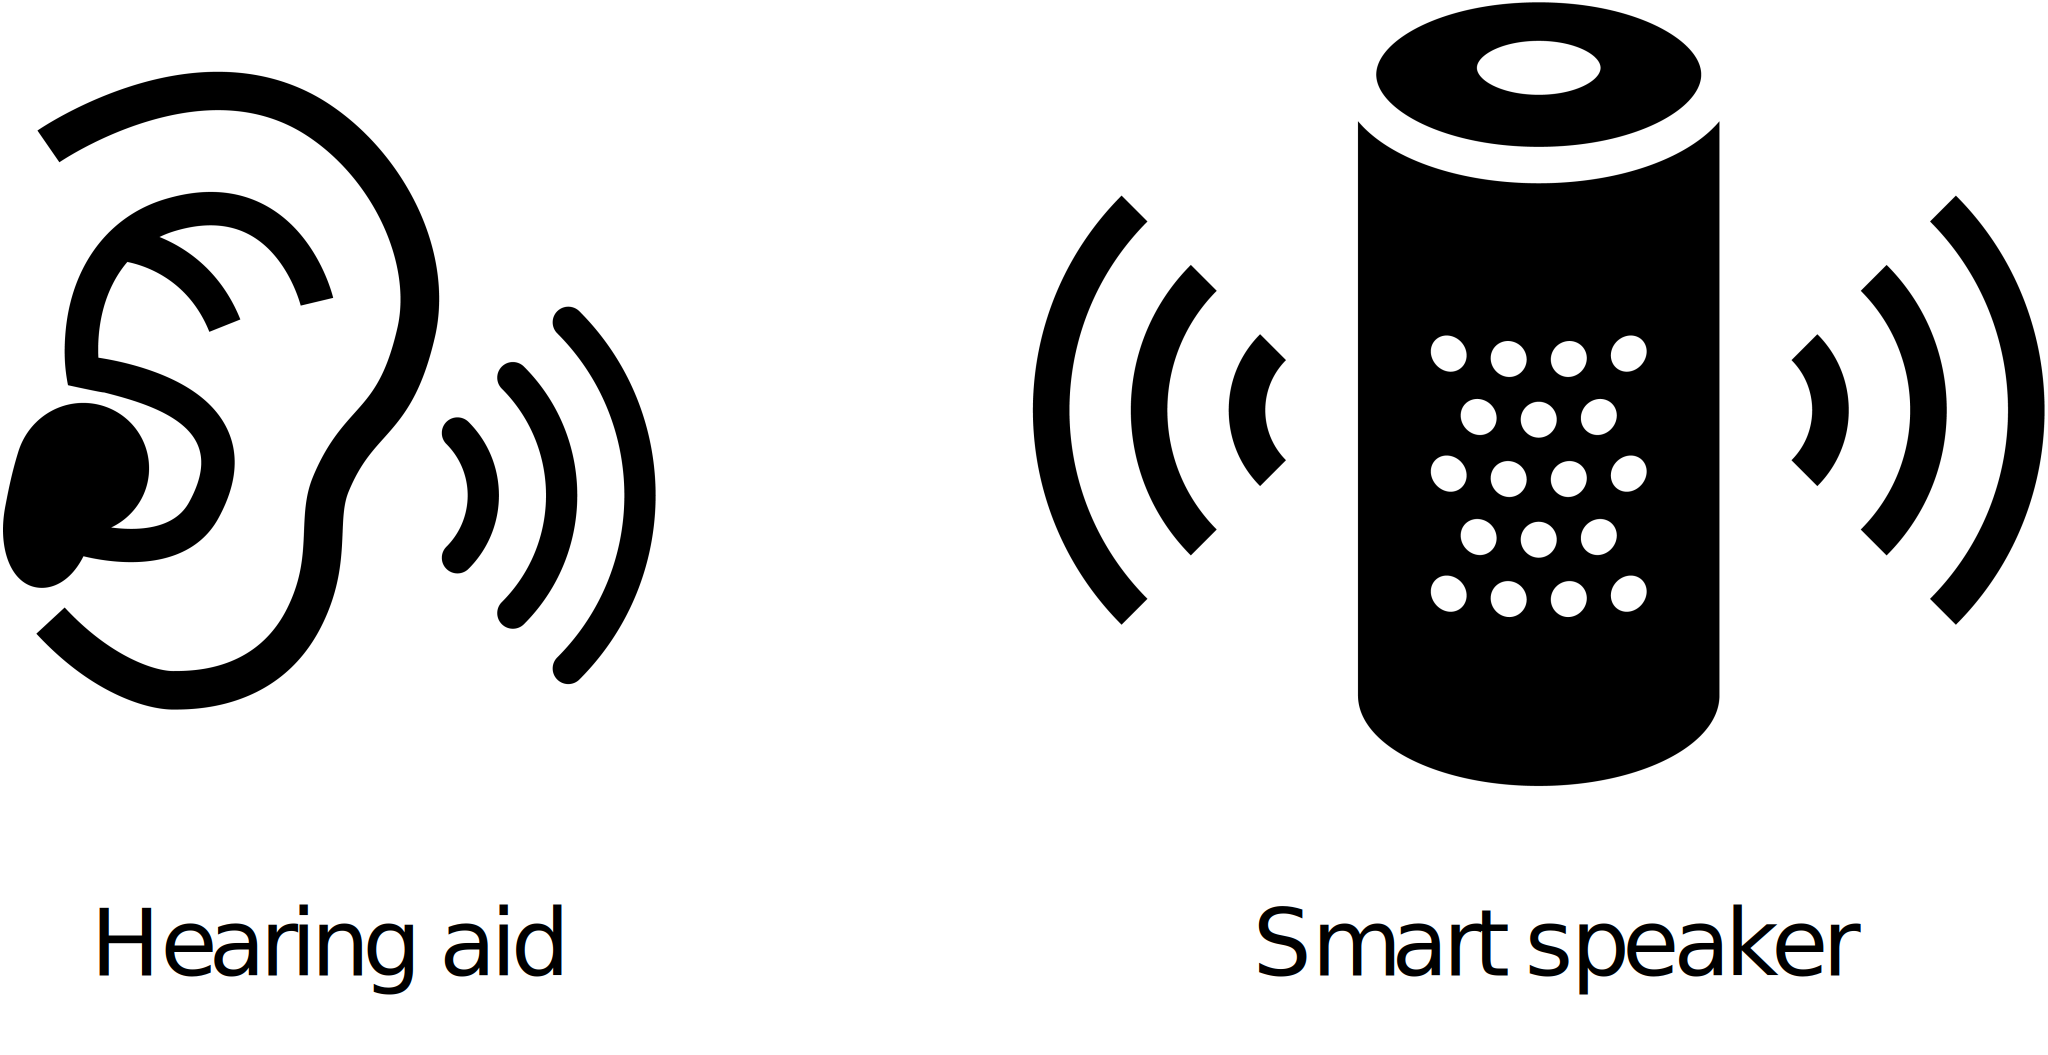
\includegraphics[width=0.7\columnwidth]{figures/using_audio_sep.pdf}
    \end{center}
    \vspace{-8pt}
	\caption{Examples of application using speech source separation.}
	\label{fig:apps}
\end{figure}
%%%%%%%%%%%%%%%%%%%%%%%%%%%%

上記のように,音源分離技術は\blue{近年ニーズが高まっており}\red{歴史的にみても非常に重要な技術として長年研究されており},これらのタスクを満足するには高精度な音源分離手法が求められる.
この経緯から1990 年代から今日まであらゆる音源分離手法が提案されてきた.
その音源分離手法の中でも,マイクロホンや音源の位置等の事前情報
が無いという条件下で,複数の信号源が混合した混合音から,混合前の分離音を推定するような分離手法をブラインド音源分離(blind source separation: BSS)\cite{BSS}という.
Fig.~\ref{fig:bss} はBSSの概要を示しており,未知の混合系$\bm{A}$(マイクロホンや音源位置や部屋の形状及び材質などに依存して変化)から混合信号が生成される.これに対して混合系$\bm{A}$の逆系である分離系$\bm{W}$を推定し,
\blue{混合系{$\bm{A}$}}観測信号$\bm{X}$に適用することで混合前の音源を推定する.
%%%%%%%%%%%%%%%%%%%%%%%%%%%%
\begin{figure}[t]
    \vspace{4pt}
    \begin{center}
        \includegraphics[width=0.9\columnwidth]{figures/BSS.pdf}
    \end{center}
    \vspace{-8pt}
	\caption{Overview of BSS.}
	\label{fig:bss}
\end{figure}
%%%%%%%%%%%%%%%%%%%%%%%%%%%%

特に,観測マイクロホン数が音源数以上となる\red{収録条件のことを優決定条件と呼ぶ.この条件下での}音源分離には,音源信号間の統計的独立性の仮定に基づく手法が広く用いられている.
独立成分分析(independent component analysis: ICA)\cite{ICA}は,優決定条件下の\red{BSS}に広く適用されている代表的な手法である.
音響信号の混合問題では一般的に残響の影響を受けて,瞬時混合ではなく時間畳み込み混合となることから,直接ICAを時間領域の観測信号に適用してもBSSを達成することは不可能である.
そこで,観測信号を時間周波数領域に変換することで周波数毎の瞬時混合として混合系をモデル化し,周波数毎にICAを適用する\red{時間}周波数領域ICA(frequency-domain ICA: FDICA)\cite{FDICA}が提案された.
ここで,ICAは一般に推定分離信号の順番が不定であり,FDICAは周波数毎に独立なICAによるBSSを行うため,分離信号の順番が周波数毎にばらばらになってしまう問題が生じる.
FDICAにおいて,周波数毎の分離信号を正しい順番に並び替える問題は一般に\red{「パーミュテーション問題」}と呼ばれており,過去には隣接周波数の時系列強度(音源アクティベーション)の相関を用いたパーミュテーション解決法\red{~\cite{COR,Permutation_solverBSS}},
マイクロホンの相対的な位置情報を既知として音源到来方位を計算し,パーミュテーション解決の手掛かりとする手法~\cite{DOA},及びその両者を組み合わせた手法~\cite{DOACOR}が提案されている.
また,近年ではFDICAに対して音源の時間周波数成分の共起関係を新たに仮定して,パーミュテーション問題を可能な限り回避しながら周波数毎の分離信号を推定する手法が登場している.
例えば,独立ベクトル分析(independent vector analysis: IVA)\cite{IVA1,IVA2}は,同一音源の周波数成分の共起を仮定しており,
非負値行列因子分解(nonnegative matrix factorization: NMF)\cite{NMF}とIVAを組み合わせた独立低ランク行列分析(independent low-rank matrix analysis: ILRMA)\cite{ILRMA1,ILRMA2}は同一音源の時間周波数成分の共起が低ランク構造を持つことを仮定している.


%----------------------------------------------
\section{本論文の目的}
%----------------------------------------------
前述したブラインドな音源分離手法は,パーミュテーション問題を回避しつつ,高い精度で分離するモデルへと発展を遂げてきた.
しかしながら,パーミュテーション問題の解は組み合わせ爆発を起こすことから,上記いずれの手法を用いても完璧にパーミュテーション問題を解くことは非常に難しい.
特に複数音声の混合信号や,\red{複数の調波楽器音の混合信号}における\red{頑健・}高精度なパーミュテーション問題の解決はいまだできていない.
一方で,文献~\cite{EU}では,複数音声の混合信号の分離時に正解のパーミュテーションを与えたFDICAが,ブラインドなIVAやILRMAよりも非常に高い分離精度を達成することを実験的に示している.
\red{従って,FDICAにおいて各周波数での音源分離は高精度であり,パーミュテーション問題のみが課題として残っている.}
\red{近年では,パーミュテーション問題を解決するために,深層ニューラルネットワーク(deep neural networks: DNN)を用いてサブバンドと呼ばれる局所帯域毎に,隣接した周波数のアクティベーションの相関を調べる手法~\cite{DNN_soluver}が提案されてきた.
しかし,この手法は局所帯域毎に処理をしているため,複雑なアルゴリズム構成となっており,3音源以上の音源分離を行うことは現実的には難しい.}
そこで,本論文では,\red{でもアルゴリズムが複雑化しない,}DNNを用いたデータ駆動型(教師あり)パーミュテーション解決法(以後,深層パーミュテーション解決法と呼ぶ)について\red{提案し,その妥当性について実験的に調査する}.
同時に,ブロックパーミュテーション問題に対\red{する有効性についても調査する}.
この\red{提案手法と既存手法の位置関係の概念図を}をFig.~\ref{fig:scope} に示す.
本論文では,FDICAにおけるパーミュテーション問題のみに焦点を当てており,分離信号成分の正しいパーミュテーションを予測する様に学習したDNNを用いてパーミュテーション問題を解決することを目的とする.
ここでは,DNN優決定条件下での複数音声の混合を模倣した人工的なデータと実際の音声及び音楽信号に対して,深層パーミュテーション解決法を適用することを考える.

%なお,劣決定音源分離において周波数毎のフルランク空間相関行列を推定するBSS ~\cite{FULLRANK}等でもパーミュテーション問題を解く必要が生じるため,提案手法はFDICAだけでなく,他の手法におけるパーミュテーション問題にも適用できる.
%%%%%%%%%%%%%%%%%%%%%%%%%%%%
\begin{figure}[t]
    \vspace{4pt}
    \begin{center}
        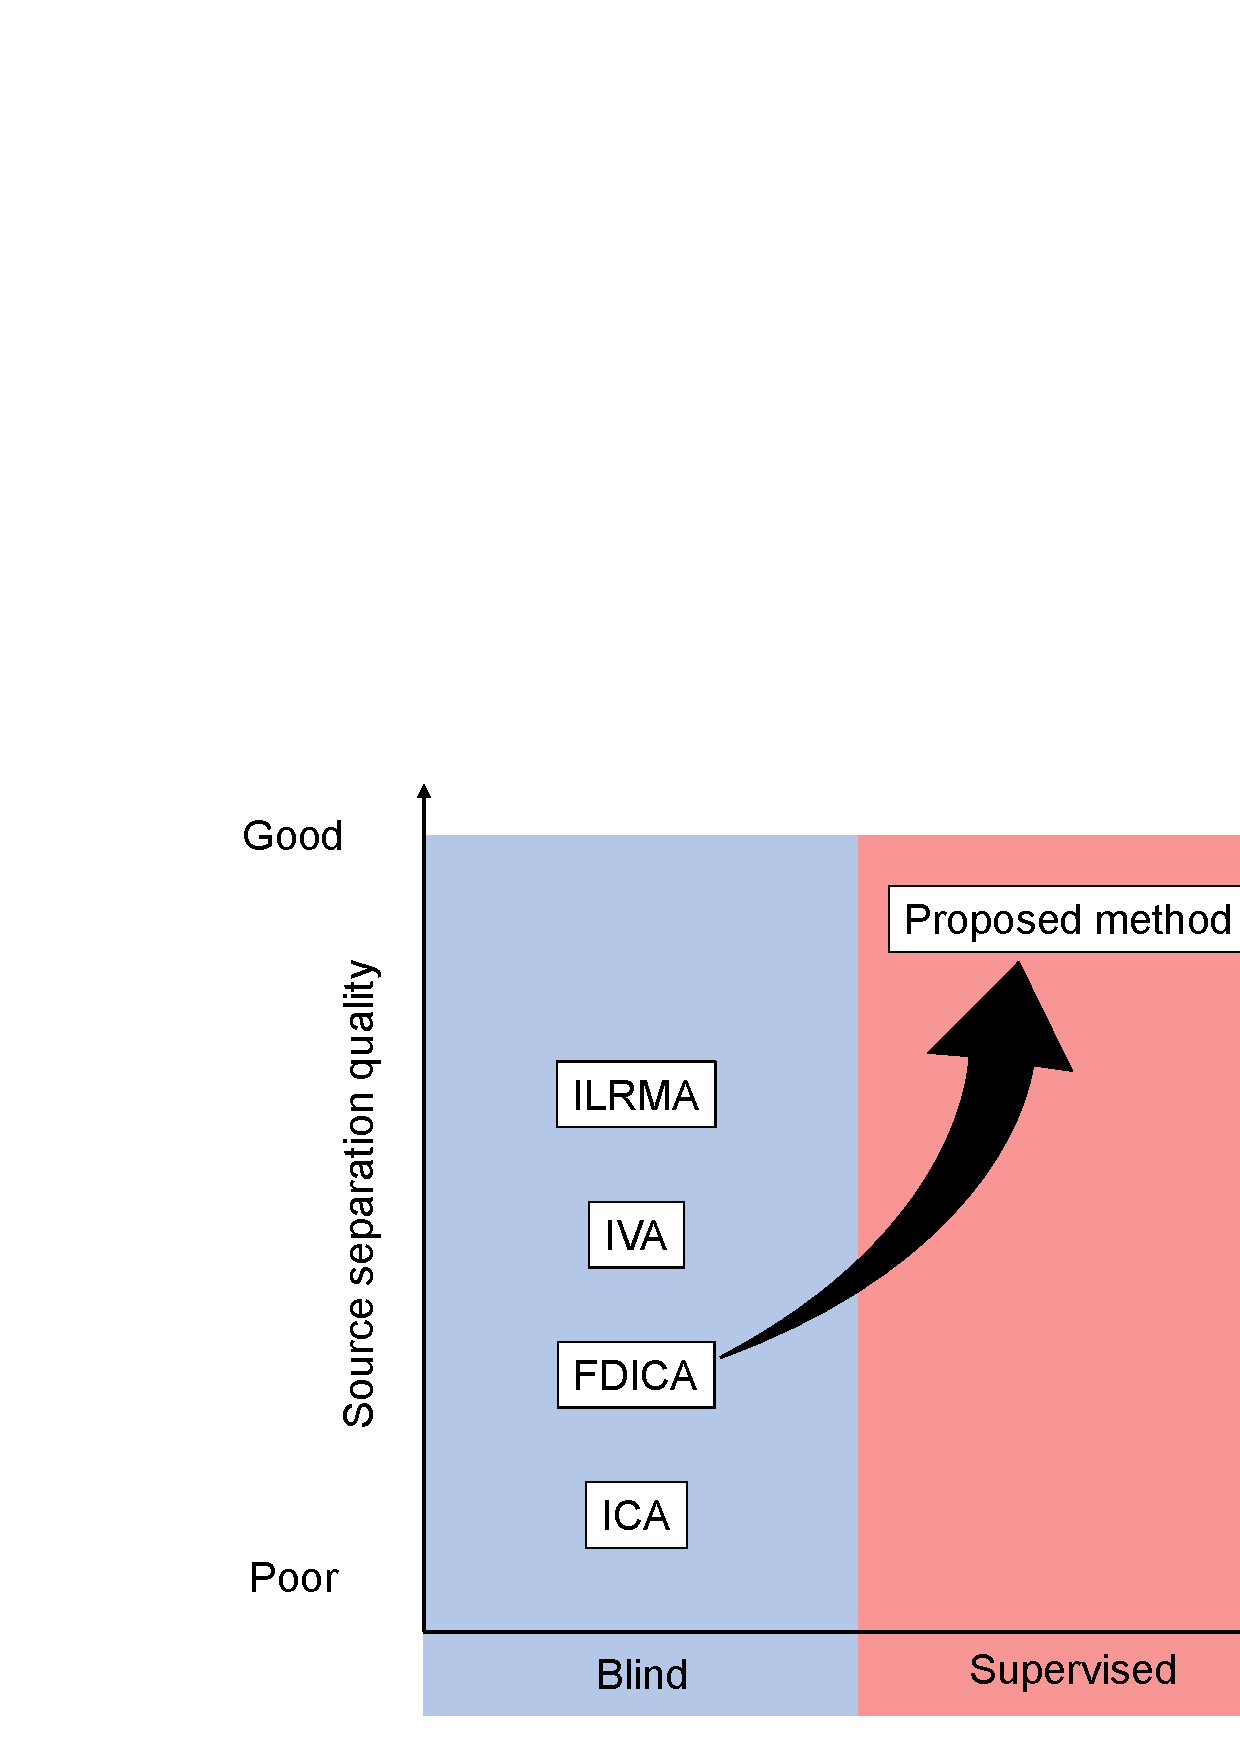
\includegraphics[width=1.0\columnwidth]{figures/chapter1/scope.pdf}
    \end{center}
    \vspace{-8pt}
	\caption{Scope of this thesis.}
	\label{fig:scope}
\end{figure}
%%%%%%%%%%%%%%%%%%%%%%%%%%%%


%--------------------------------------------
\section{本論文の構成}
%----------------------------------------------
まず,2章では,本論文の解決すべき課題であるパーミュテーション問題\red{の説明に必要となるICAの基本原理や音響信号の時間周波数領域への変換である短時間Fourier変換(short-time Fourier transform: STFT)に加え,
パーミュテーション問題を可能な限り回避するBSSのIVA及びILRMA,そして既存の深層パーミュテーション解決法について詳しく説明する.}
\red{これらは,いずれも提案手法の説明に必要となる知識である.}
3章では,本論文の提案手法である深層パーミュテーション解決法の新たなアルゴリズムの詳細について,\red{DNNの構造からパーミュテーション解決の処理までを詳細に述べる.}
4章では\blue{音声の混合信号を模倣した}人工データと実際の音声及び音楽信号に対する音源分離実験を行い,提案深層パーミュテーション解決法の性能の検証を行う.
最後に5章では, すべての章を総括した結言を述べる.




%%%%% 第2章 %%%%%
\chapter{従来手法}
\label{chap:conv}

%----------------------------------------------
\section{まえがき}
%----------------------------------------------
まず,\ref{sec:ica}節では,提案手法において必要な基礎理論を説明するため,音源分離手法のICAについて説明する.
\ref{sec:stft}節では,音響信号処理でよく用いられる,短時間フーリエ変換(short-time Fourier transform: STFT)について説明する.
\ref{sec:formularization}節では,時間周波数領域における音源信号及びBSSの定式化を導入する.
\ref{sec:fdica}節では,音源分離手法の1つであるFDICAについて説明する.
\ref{sec:pp}節では,パーミュテーション問題と呼ばれるFDICAに伴う課題の説明と,既存のパーミュテーション解決法について説明する.
\ref{sec:ivailrma}節では,既存の深層パーミュテーション解決法について説明する
%----------------------------------------------
\section{ICAの基本原理}
\label{sec:ica}
%----------------------------------------------
%----------------------------------------------
\subsection{信号源の混合モデルと分離方法}
%----------------------------------------------

本項では,BSSの基礎であるICAについて説明する.
今,2つの信号源$s_1(l)$及び$s_2(l)$があり,その混合信号を2つのマイクロホンで観測するという状況を考える.
ここで,$l = 1, 2, \cdots , L$は離散時間インデクスを示す.
マイクロホンで観測された信号を
$x_1(l)$及び$x_2(l)$とすると,2つの信号源の混合現象は次の連立方程式でモデル化できる.
\begin{eqnarray}
  \begin{cases}
    x_1(l) = a_{11}s_1(l) + a_{12}s_2(l)  \label{f:a1}\\
    x_2(l) = a_{21}s_1(l) + a_{22}s_2(l)  \label{f:a2}
  \end{cases}
\end{eqnarray}
ここで,信号の伝搬を表す係数$a_{mn}$は,時刻$t$には依存せず常に一定であると仮定する.
即ち,信号源の位置及びマイクロホンの位置が動かないことを仮定している.
また,$n = 1, 2, \cdots , N$,及び$m =
1, 2, \cdots , M $はそれぞ音源及びチャネルのインデクスを示す.
伝搬係数$a_{mn}$をまとめた行列を以下のように定義する.
\begin{align}
    \bm{A} = \begin{pmatrix}
    a_{11}  & a_{12}  \\
    a_{21}  & a_{22}  \\
    \end{pmatrix}
\end{align}
この行列$\bm{A}$は混合行列と呼ばれる.
観測信号ベクトル$\bm{x}(l) = (x_1(l),x_2(l))^T$
信号源ベクトル$\bm{s}(l) = (s_1(l),s_2(l))^T$
及び混合行列$\bm{A}$を用いて,式(\ref{f:a1})及び(\ref{f:a2})の連立方程式は次式のように書き直せる.
\begin{align}
    \bm{x}(l) = \bm{A}\bm{s}(l) \label{f:x}
\end{align}
ここで,$\cdot^\mathrm{T}$ はベクトルや行列の転置を表す.
分離信号を$y(l) = (y_1(l),y_2(l))^T$,分離行列を$\bm{W}$とそれぞれ定義すると,音源分離は以下のように表される.
\begin{align}
    \bm{y}(l) = \bm{W}\bm{x}(l)
\end{align}
このとき,混合行列$\bm{A}$の逆行列が存在する($\bm{A}$が正則)ならば,$\bm{W}=\bm{A}^{-1}$となるように$\bm{W}$を選択することで,信号源$s(l)$を推定することができる.
\begin{align}
    \bm{y}(l) &= \bm{W}\bm{x}(l)\\
    &= \bm{A}^{-1}\bm{x}(l)\\
    &= \bm{A}^{-1}\bm{A}\bm{s}(l)\\
    &= \bm{s}(l)
\end{align}

このように,混合行列$\bm{A}$の逆行列を推定することで,音源分離を達成することができる.
しかしながら,音源やマイクロホンの位置関係が未知であるBSSにおいては,混合行列$\bm{A}$もまた未知である.
そこで,ICAでは,信号源の混合モデル式(\ref{f:x})の仮定の他に,信号そのものの統計的なモデル($p(s_1)$ 及び$p(s_2)$に対する仮定)を導入することで,分離フィルタ$\bm{W}$を推定する.

%--------------------------------------------
\subsection{統計的独立性}
%----------------------------------------------
ICA による信号源分離を理解する上での重要な概念として,統計的独立性がある.
今,信号源$s_1(l)$及び$s_2(l)$を確率変数として扱い,それらの生成モデルを$p(s_1)$及び$p(s_2)$と定義する.
通常,各信号源($s_1(l)$及び$s_2(l)$)は互いに無関係であり,$s_1(l)$から$s_2(l)$を推定することはできないはずである.
そのため,$s_1(l)$と$s_2(l)$は互いに統計的に独立とみなすことができ,次式が成立する.
\begin{align}
    p(s_1,s_2) = p(s_1)p(s_2) \label{f:y}
\end{align}
同様に,理想的な分離フィルタが推定できれば,分離信号$y_n(l)$も統計的に独立であるため,次式が成立する.
\begin{align}
    p(y_1,y_2) = p(y_1)p(y_2)
\end{align}
ここで,$p(y_1)$及び$p(y_2)$はそれぞれ分離信号$y_1(l)$及び$y_2(l) $の生成モデルであり,$p(y_1, y_2)$は同
時分布である.
従ってICAによるBSSは,式(\ref{f:y})が成立するような分離フィルタ$\bm{W}$を推定する問題であると解釈できる.
上記の問題を定式化すると,次式のように書き表せる.
\begin{align}
   \argmin_{\bm{W}} \mathfrak{I}(\bm{W})
\end{align}
\begin{align}
 \mathfrak{I}(\bm{W}) = \mathfrak{D}_{KL}[p(y_1,y_2)||p(y_1)p(y_2)] \label{f:cost}
\end{align}
ここで,$\mathfrak{D}_{KL}[p(s)||q(s)]$はカルバックライブラ・ダイバージェンス(Kullback--Leibler divergence: KL divergence)と呼ばれ,2つの分布間($p(s)$及び$q(s)$)の距離を測る関数として次式のように定義される.
\begin{align}
\mathfrak{D}_{KL}[p(s)||q(s)] = \int{p(s){\rm log}~\frac{p(s)}{q(s)}}ds \label{f:kld}
\end{align}
また,分離フィルタ$\bm{W}$で線形変換する前($\bm{x}$)と後($\bm{y}$)の確率変数を考えたとき,それぞれ
の同時分布$p(\bm{y}) = p(y1,y2) $と$p(\bm{x}) = p(x1,x2)$の間には,次式が成立する.
\begin{align}
    p(\bm{y}) = \frac{1}{|\mathrm{det}~\bm{W}|}p(\bm{x}) \label{f:detw}
\end{align}
式(\ref{f:kld})及び(\ref{f:detw})を用いて式(\ref{f:cost})を変形すると,最終的な最小化関数$\mathfrak{I}(\bm{W})$は以下のように書ける.
\begin{align}
\begin{split}
  \mathfrak{I}(\bm{W}) &= \int_{-\infty}^{\infty} \int_{-\infty}^{\infty} p(x_1,x_2){\rm log}~p(x_1,x_2)dx_1 dx_2 - {\rm log}~|\mathrm{det}~\bm{W}|\\
  &\quad -\int_{-\infty}^{\infty} p(y_1){\rm log}~p(y_1)dy_1 - \int_{-\infty}^{\infty} p(y_2){\rm log}~p(y_2)dy_2    \label{f:newcost}
\end{split}
\end{align}
ICAでは式(\ref{f:newcost})を$\bm{W}$について最小化することで,信号源を分離する.

%----------------------------------------------
\section{STFT}
\label{sec:stft}
%----------------------------------------------
%%%%%%%%%%%%%%%%%%%%%%%%%%%%
\begin{figure}[t]
    \begin{center}
        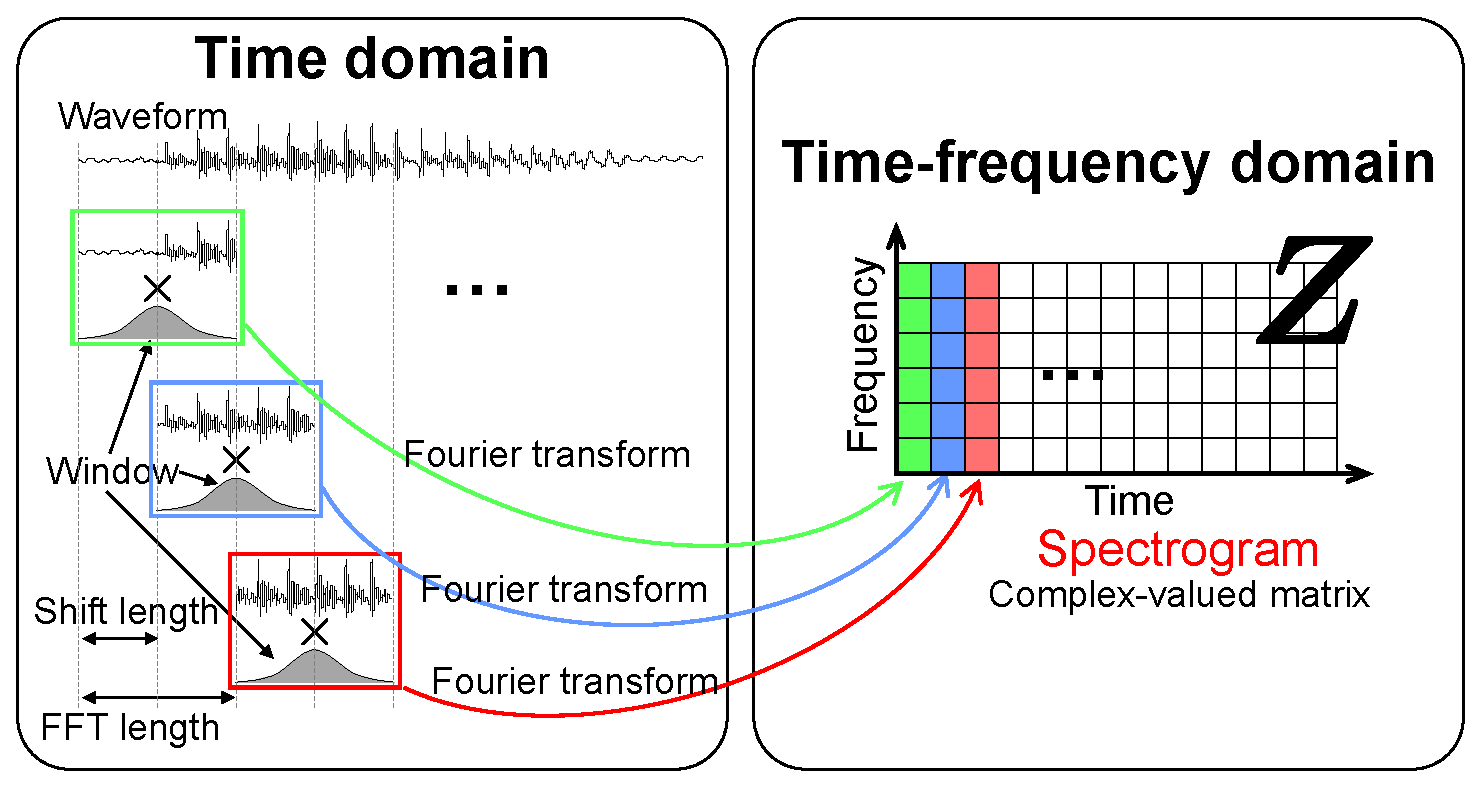
\includegraphics[width=0.95\columnwidth]{figures/stft.eps}
    \end{center}
    \vspace{-8pt}
	\caption{Mechanism of STFT.}
	\label{fig:stft}
\end{figure}
%%%%%%%%%%%%%%%%%%%%%%%%%%%%
STFTはFig.~\ref{fig:stft}に示すような時
間的に変化するスペクトルを表現するための手法である.
STFT の分析窓関数の長さ及びシフト長をそれぞれ$Q$及び$\tau$としたとき,時間領域の信号
$z(l)$の$j$番目の短時間区間(時間フレーム)の信号は次式で表される.
\begin{align}
    \bm{z}^{(j)} &= \left(z\left((j-1)\tau+1\right), z\left((j-1)\tau+2\right), \cdots , z\left((j-1)\tau+Q\right) \right)^{T}\\
    &= \left(
    z^{(j)}(1),z^{(j)}(2),\cdots , z^{(j)}(q), \cdots , z^{(j)}(Q)
    \right)^{T}~\in \mathbb{R}^{Q}
\end{align}
ここで,$j= 1, 2, \cdots , J$及び$q= 1, 2, \cdots , Q$は,それぞれ時間フレーム及び時間フレーム内のサン
プルを示す.また,セグメント数$J$は次式によって与えられる.
\begin{align}
    J = \frac{L}{\tau}
\end{align}
また,各時間フレームの信号のSTFTは次式のようにして求められる.
\begin{align}
\bm{Z}= {\rm STFT}_{\bm{\omega}}(\bm{z})~\in \mathbb{C}^{I \times J}
\end{align}
また,スペクトログラム$\bm{Z}$の$(i, j)$ 番目の要素は次式で表される.
\begin{align}
    z_{ij}= \sum_{q=1}^{Q}\omega(q)z^{(j)}(q){\rm exp}\left\{\frac{-\iota2\pi(q-1)(i-1)}{F}\right\}
\end{align}
ここで$F$は$\lfloor \frac{F}{2}\rfloor+1 =I$を満たす整数($\lfloor \cdot \rfloor$は床関数)を,$i= 1, 2, \cdots , I$は周波数ビンのインデクスを,
$\iota$は虚数単位を,$\bm{\omega}$は分析窓関数を示している.
このように,時間領域の信号は一定幅の短時間ごとに分析窓関数を乗じて離散フーリエ変換を行うことで,横軸が時間,縦軸が周波数のスペクトログラムと呼ばれる複素行列$\bm{Z}$で表すことができる.

%----------------------------------------------
\section{周波数領域におけるBSSの定式化}
\label{sec:formularization}
%----------------------------------------------
今一度,音源数と観測チャネル数(マイクロホン数)をそれぞれ$N$及び$M$とする.
また,各観測音源信号をSTFTすることで得られる,各時間周波数における音声信号,混合信号,及び分離信号をそれぞれ
\begin{align}
  \bm{s}_{ij} &= \left(
	s_{ij,1},s_{ij,2}, \cdots, s_{ij,n}, \cdots, s_{ij,N} 
  \right)^\mathrm{T}~\in \mathbb{C}^{N}\\
  \bm{x}_{ij} &= \left(
      x_{ij,1},x_{ij,2},  \cdots, x_{ij,m}, \cdots  , x_{ij,M} 
  \right)^\mathrm{T}~\in \mathbb{C}^{M} \\
  \bm{z}_{ij} &= \left(
      z_{ij,1},z_{ij,2},  \cdots, z_{ij,n}, \cdots  , z_{ij,N} 
  \right)^\mathrm{T}~\in \mathbb{C}^{N}
\end{align}
と表す.
ここで,$i= 1, 2, \cdots , I$,$j = 1, 2, \cdots , J$,$n = 1, 2, \cdots , N$,及び$m =
1, 2, \cdots , M $はそれぞれ周波数,時間,音源,チャネルのインデクスを示す.
また,複素スペクトログラム行列$\bm{S}_{n} \in \mathbb{C}^{I\times J}$, $\bm{X}_{m} \in \mathbb{C}^{I\times J}$及び$\bm{Z}_{n} \in \mathbb{C}^{I\times J}$の成分をそれぞれ
$s_{i, j, n}$, $x_{i, j, m}$及び$z_{i, j, n}$ と表す.

%----------------------------------------------
\section{FDICA}
\label{sec:fdica}
%----------------------------------------------
\ref{sec:ica}節で説明したように,ICAとは,観測信号が独立信号の線形結合として観測される場合に,各信号間の独立性を最も高めるように線形分離行列を推定することでBSSを実現する手法である.
しかし,実際に観測される音声信号には残響の影響を受けており,線形時不変なインパルス応答が畳み込まれて混合される.
インパルス応答の畳み込みは残響長$R$を用いて次式のように表される.
\begin{align}
  \bm{x}(l) = \sum_n \sum_{l^{'}=0}^{R-1} \tilde{\bm{a}}_n(l^{'}) \bm{s}_n(l-l^{'})
  \label{f:tatami}
\end{align}
ここで,$\tilde{\bm{a}}_n(l)$は,音源$n$に対する畳み込み混合係数ベクトル(音源$n$からマイクロフォン$m$までのインパルス応答をまとめたもの)である.
これを分離するためには逆畳み込みフィルタを推定することが必要となる.
一般的に逆畳み込みフィルタの推定は容易ではないことから,時間領域でのICAによるBSSは困難である.
この問題を解決するために,式(\ref{f:tatami})の時間領域における畳み込み混合を,STFTによって周波数領域上での瞬時混合に変換し,時間周波数領域で周波数毎にICAを行うFDICAが提案された.

FDICAでは,周波数毎の時不変な混合行列 $\bm{A}_{i} = (\bm{a}_{i, 1} ~\bm{a}_{i, 2} ~\cdots ~\bm{a}_{i, n}~\cdots,\bm{a}_{i, N} )\in \mathbb{C}^{M\times N}$を定義し,混合信号が次式で表現できると仮定する.
\begin{align}
 \bm{x}_{ij} = \bm{A}_i\bm{s}_{ij}
\end{align}
この混合モデルは,STFTの窓長が室内残響よりも長い場合にのみ成立する.
以後,決定的な系($M=N$)を仮定すると,混合行列$\bm{A}_{i}$が正則であれば,分離行列$\bm{W}_i=\bm{A}_i^{-1}=(\bm{w}_{i,1}~\bm{w}_{i,2}~ ...~ \bm{w}_{i, n}~ ... ~\bm{w}_{i, N})^{\mathrm{H}}$を用いて,分離信号を次式で表せる.
\begin{align}
 \bm{z}_{ij} = \bm{W}_{i}\bm{x}_{ij} \label{eq:sep}
\end{align}
ここで,$\cdot^\mathrm{H}$はベクトルや行列のエルミート転置を示す.
分離行列の行ベクトルである$\bm{w}_{i,n}\in\mathbb{C}^M$は,周波数$i$において,観測信号から$n$番目のみの音源へ変換する分離フィルタである.
このようにFDICAでは,観測信号$\bm{x}_{ij}$の各周波数ビンに対しそれぞれ独立にICA を適用することで,周波数毎の分離行列$\bm{W}_{i}$を全周波数にわたって推定することで音源分離を行う.

%----------------------------------------------
\section{パーミュテーション問題とその解決}
\label{sec:pp}
%----------------------------------------------
FDICA中で周波数毎に適用しているICAは,音源間の統計的独立性のみに基づいて分離行列を推定するため,分離音源の周波数毎のスケール及び順番に関しては不定である.
従って,FDICAの推定分離行列を$\hat{\bm{W}}_i$とすると,次式のような不定性が残る.
\begin{align}
	\hat{\bm{W}}_{i} &= \bm{D}_{i}\bm{P}_{i}  \bm{W}_{i}
\end{align}
ここで,$\bm{P}_i \in \{0, 1\}^{N \times N}$は分離行列$\bm{W}_{i}$の行ベクトル$\bm{w}_{i, n}$の順番を入れ変えうるパーミュテーション行列(置換行列)である.
$\bm{D}_i \in \mathbb{R}^{N \times N}$は,$\bm{w}_{i,n}$のスケールを変化させる可能性のある対角行列である.
すなわち,FDICAで推定される分離信号
\begin{align}
\bm{y}_{ij} &= \hat{\bm{W}}_i\bm{x}_{ij} \\
&=\left( y_{ij,1},y_{ij,2}, \cdots, y_{ij,n}, \cdots, y_{ij,N} \right)^\mathrm{T}~\in \mathbb{C}^{N} \label{eq:sepSig}
\end{align}
は,推定音源の順番やスケールが周波数毎にばらばらになっている状態である.
このうち,$\bm{D}_i$によって生じるスケールの任意性は,プロジェクションバック法\cite{Matsuoka2001_PB}で復元可能である.
一方で,$\bm{P}_i$によって生じる分離信号の順番の任意性(パーミュテーション)を純粋に復元することは,組み合わせ爆発が発生するため容易ではない.
この問題は,一般的にパーミュテーション問題と呼ばれる.
パーミュテーション問題の概要をFig.~\ref{fig:permu}に示す.
ここで,FDICAで推定される分離信号$\bm{y}_{ij}$の音源毎の複素スペクト
ログラム行列を$\bm{Y}_n \in \mathbb{C}^{I \times J}$で表している.
FDICA直後の$\bm{Y}_n$に注目すると,周波数毎での音源分離は達成できている.
しかし,時間周波数構造全体としては,異なるグループの分離信号が1つの時間周波数構造に混在していることが分かる.
これがパーミュテーション問題であり,ICAの分離信号の順番に関する不定性に起因して発生している.
そのため,FDICAにはポスト処理として,分離された音源の順番を全周波数ビンにわたって正しく並べ直す必要がある.
%%%%%%%%%%%%%%%%%%%%%%%%%%%%
\begin{figure}[t]
    \begin{center}
        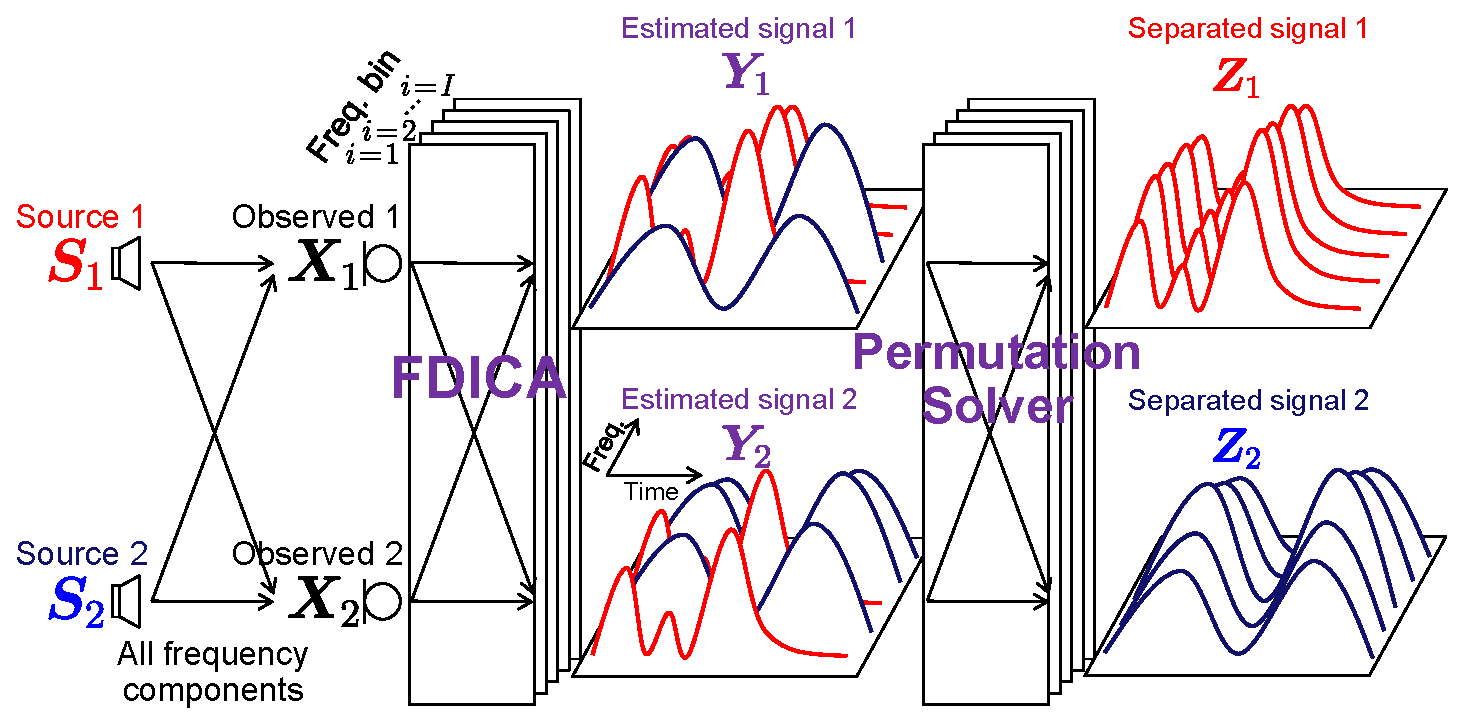
\includegraphics[width=0.95\columnwidth]{figures/permutation_image.eps}
    \end{center}
    \vspace{-8pt}
	\caption{Permutation problem in FDICA, where $N=M=2$.}
	\label{fig:permu}
\end{figure}
%%%%%%%%%%%%%%%%%%%%%%%%%%%%

パーミュテーション問題を解決して得られる分離信号は次式となる.
\begin{align}
\bm{z}_{ij} &= \bm{P}_{i}^{-1}\bm{D}_{i}^{-1}\bm{y}_{ij} \label{eq:z}
\end{align}
%本論文では,この$\bm{P}_{i}^{-1}$を推定することが目的となる.

このパーミュテーション問題を解決するために,これまでにも数々のパーミュテーション解決法が提案されてきた.
代表的な既存手法の1つに,隣接周波数の時系列強度(音源アクティベーション)の相関を用いたパーミュテーション解決法\cite{COR}がある.
これは,分離信号のパーミュテーションが正しければ,隣接した周波数アクティベーション間の相関が高くなりやすいという仮定の下で並べ替える手法である.また,離れた周波数においても,同じ音源のアクティベーション間の相関が高くなるように並び替えられている.
%り,次式のように相関を計算する.
%\begin{align}
%\Tilde{\bm{v}}_{i}(n) &=  \frac{1}{J}\sum_{j=0}^{J} |\bm{y}_{i,j,n}| \\
% {\rm sim}(i) &= \sum_{n\neq m} \frac{\Tilde{\bm{v}}_{i}(n) \cdot \Tilde{\bm{v}}_{i}(m)}{\|
% \Tilde{\bm{v}}_{i}(n)\|~\| \Tilde{\bm{v}}_{i}(m)\|}
%\end{align}
%ここで,$\cdot$は内積を表しており,
他にも,マイクロホンの相対的な位置情報を既知として音源到来方位を計算し,パーミュテーション解決の手掛かりとする手法 \cite{DOA}および両者を組み合わせたパーミュテーション解決法も提案されている.
しかしながら,パーミュテーション問題の解は組み合わせ爆発を起こすことから,上記いずれの手法を用
いても完璧にパーミュテーション問題を解くことは非常に難しく,とくに複数音声の混合信号における高精
度なパーミュテーション問題の解決はいまだできていない.

%----------------------------------------------
\section{深層パーミュテーション解決法}
\label{sec:ivailrma}
%----------------------------------------------

近年では,DNNを用いたパーミュテーション問題解決法が登場している.観測された混合信号$\bm{X}_n$にFDICA適用すると,パーミュテーション問題が生じた分離信号$\bm{Y}_n$が得られる.
これらのパワースペクトログラム$|\bm{Y}_n|^{.2}$から全周波数帯域中の局所的な狭帯域(サブバンド)を定義し,サブバンド毎にデータをDNNに入力し,パーミュテーションを解決する.
サブバンド毎に参照周波数を定義し,その近傍周波数が参照周波数に対して同一音源か否かを判断し,同一音源である場合はDNNの出力として「0」を出力し,同一音源でない場合はDNNの出力として「1」を出力する.2つの周波数これらの推定処理をFig.~に示す.
参照周波数と近傍周波数を($i,i+\omega$),短時間時系列パワー(長さ$\tau $)を以下のように集める.
\begin{align}
  %\bm{d}_{i, \omega, \gamma} &= ({\bm{r}_{i, \gamma, 1}}^\mathrm{T}, {\bm{r}_{i, \gamma, 2}}^\mathrm{T}, {\bm{g}_{i, \omega, \gamma, 1}}^\mathrm{T}, {\bm{g}_{i, \omega, \gamma,2}}^\mathrm{T} )^\mathrm{T}~\in \mathbb{R}_{\geq 0}^{4\tau \times 1},\label{eq:DNNinputVec}\\
  \bm{d}_{i, \omega, \gamma} &= ({\tilde{\bm{r}}_{i, \gamma}}^\mathrm{T}, {\tilde{\bm{g}}_{i, \omega, \gamma}}^\mathrm{T} )^\mathrm{T}~\in \mathbb{R}_{\geq 0}^{4\tau \times 1} \label{eq:DNNinputVec}\\
  \tilde{\bm{r}}_{i,\gamma} &= ({\bm{r}_{i, \gamma, 1}}^\mathrm{T}, {\bm{r}_{i, \gamma, 2}}^\mathrm{T} )^\mathrm{T}~\in \mathbb{R}_{\geq 0}^{2\tau \times 1} \label{eq:DNNinputVecRtilde}\\
  \bm{r}_{i, \gamma, n} &= ( |y_{i, (\gamma-1) \eta+1, n}|^2, |y_{i, (\gamma-1) \eta+2, n} |^2, 
  \cdots, |y_{i, (\gamma-1) \eta+\tau, n}|^2 )^\mathrm{T}~\in \mathbb{R}_{\geq 0}^{\tau \times 1}  \label{tau1}\\
  \tilde{\bm{g}}_{i,\omega,\gamma} &= ({\bm{g}_{i, \omega, \gamma, 1}}^\mathrm{T}, {\bm{g}_{i, \omega, \gamma, 2}}^\mathrm{T} )^\mathrm{T}~\in \mathbb{R}_{\geq 0}^{2\tau \times 1} \label{eq:DNNinputVecGtilde}\\
  \bm{g}_{i,\omega, \gamma, n} &= ( |y_{i+\omega, (\gamma-1) \eta+1, n}|^2, |y_{i+\omega, (\gamma-1) \eta+2, n}|^2,\cdots, |y_{i+\omega, (\gamma-1) \eta+\tau, n}|^2 )^\mathrm{T}~\in \mathbb{R}_{\geq 0}^{\tau \times 1} \label{tau2}
\end{align}
  ここで,行列の $|\cdot|^{.2}$ は,要素ごとの絶対値の二乗を返す.
  また,$\omega=-\Omega, -\Omega+1, \cdots, -1, 0, 1, \cdots, \Omega$は,$\bm{r}_{i,\gamma,n}$と$\bm{g}_{i,\omega,\gamma,n}$の周波数の差であり,$\eta$は,短時間セグメントの時間軸に沿ったストライド幅,$\gamma=1, 2, \cdots, \Gamma$は,短時間セグメントのインデクスである.
  なお,$\Gamma$は,短時間のアクティベーションの長さ$\tau$ とストライド幅$\eta$によって決まる.
  ベクトル $\bm{r}_{i,\gamma,n}$ は,参照周波数$i$の短時間時系列パワーに対応し,ベクトル $\bm{g}_{i,\omega,\gamma,n}$は,Fig.~\ref{fig:input}に示すように,隣接又は局所周波数$i+\omega$ の短時間時系列パワーに対応する.
  DNNの入力ベクトルは,(\ref{eq:DNNinputVec})を正規化したものとして次のようにして表す.
\begin{align}
  \tilde{\bm{d}}_{i, \omega, \gamma} &=\frac{\bm{d}_{i, \omega, \gamma} }{ \|{\bm{d}_{i, \omega, \gamma} }\|_2}~\in \mathbb{R}_{\geq 0}^{4\tau \times 1}  \label{eq:input}
\end{align}
提案するDNNモデルは,0または1を出力する2値分類器である.
推定結果が「0」の場合は,$\bm{r}_{i,\gamma, 1}$と$\bm{g}_{i,\omega,\gamma, 1}$が同一音源であることを意味し,同様に$\bm{r}_{i,\gamma, 2}$と$\bm{g}_{i,\omega,\gamma, 2}$も同一音源である.
一方,推定結果が「1」の場合は$\bm{r}_{i,\gamma, 1}$と$\bm{g}_{i,\omega,\gamma, 1}$(同様に$\bm{r}_{i,\gamma, 2}$と$\bm{g}_{i,\omega,\gamma, 2}$)が異なる音源成分であることを意味している.
これらの推定処理をFig.~\ref{fig:local_dnn}に示す.DNNの予測結果は次のように表せれる.
\begin{align}
  q_{i,\omega,\gamma} = \mathrm{DNN}\left(\tilde{\bm{d}}_{i,\omega,\gamma}\right) \in \{0, 1\}
\end{align}
この結果を時間方向にずらして,全時間フレームに対するDNNの予測処理を走査する.そして,DNNの予測結果を時間軸に対して多数決処理を行うことで,より信頼性の高いサブバンドベクトルを取得する.
サブバンドベクトルは,基準周波数$i$をシフトすることにより全周波数で推定する.ただ,各サブバンドベクトル内の2値は(「0」及び「1」)は異なる意味を持つ可能性がある.これはサブバンド内の周波数成分が.
参照周波数の成分と同一音源か否かを示しているに過ぎず,参照周波数の変化を共に,対応音源が変化する.2音源でサブバンドベクトル内の値が「1」,つまり同一音源ではない場合は,必然的にもう一方の音源となる.ただ,3音源以上になるとサブバンドベクトル内の値が「1」の時,残りのどの音源を一致するのかが判断できない.
そのため,3音源以上になると組み合せ爆発を起こしてしまい,計算量の観点から3音源以上の音源分離は難しい.

%----------------------------------------------
\section{本章のまとめ}
%----------------------------------------------
本章では,提案手法において必要となる基礎理論および各種従来手法について説明した.
次章以降では,より簡潔に精度の良いのBSSを達成するために\ref{sec:fdica}節で導入したFDICAのポスト処理として,DNNに基づくパーミュテーション解決法を新たに提案する.


















%%%%% 第3章 %%%%%

\chapter{提案手法}
\label{chap:proposed}

%----------------------------------------------
\section{まえがき}
%----------------------------------------------
前章では,\red{音響信号のBSSにおいて重要な}FDICA\blue{に伴い生じる}\red{の}パーミュテーション問題\blue{と従来の深層}\red{について詳しく述べた.また,音源モデルに基づきパーミュテーション問題を回避する手法や,近年提案された深層}パーミュテーション解決法について説明した.
\red{さらに,既存の深層パーミュテーション解決法では,音源数$N$の増加に伴ってアルゴリズムが極端に複雑になってしまう課題について述べた.}
本章では,\blue{組み合せ爆発を起こすことのない,DNNを用いたデータ駆動型パーミュテーション解決法を新たに提案する.}
\red{音源数$N$が増加した場合でもアルゴリズムが複雑化することのない深層パーミュテーション解決法を新たに提案する.}
\blue{{\ref{sec:moti}}節では,IVAやILRMAのようなブラインド(教師無し)なパーミュテーション解決法における課題と従来の深層パーミュテーション解決法における課題を述べ,データ駆動型の教師ありパーミュテーション解決法を新たに提案する動機について明らかにする.}
\red{まず\ref{sec:moti}節では,BSSにおいて深層学習を用いてパーミュテーション問題の解決を目指す動機について述べる.}
\ref{sec:in-out}節及び\ref{sec:model}節で\red{は},\blue{提案}\red{本論文で提案する深層}パーミュテーション解決法\blue{における}\red{の}DNNモデルの入出力及び\red{ネットワーク}構造を\red{それぞれ}説明する.
\ref{sec:loss}節及び\ref{sec:maj}節では,誤差逆伝播に用いる損失\red{関数}の取り方と\blue{パーミュテーション行列の並び替えに用いる}\red{パーミュテーション行列を正確に推定するモデルを学習するための}\blue{ラベルの取得方法}\red{入力データ及び正解データ(ラベル)の取得方法}を\red{それぞれ}説明する.
\ref{sec:3matome}節で本章のまとめを述べる.

%----------------------------------------------
\section{動機}
\label{sec:moti}
%----------------------------------------------
%%%%%%%%%%%%%%%%%%%%%%%%%%%%
\begin{figure}[t]
    \begin{center}
        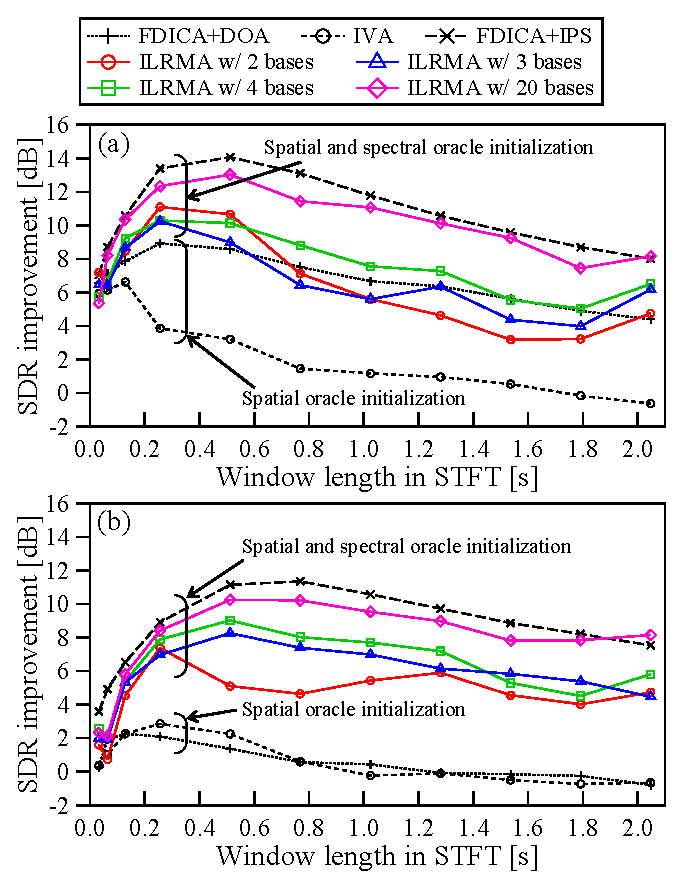
\includegraphics[width=0.8\columnwidth]{figures/SpeechE2AJR2_opt12+note.eps}
    \end{center}
    \vspace{-8pt}
	\caption{Average source separation results for speech signals using random initialization: (a) E2A (\red{$T_{60} = 300$~ms}) and (b) JR2 (\red{$T_{60}=470$~ms}) impulse responses. \red{For details of this figure, see~\cite{EU}.}}
	\label{fig:kitamura_es}
\end{figure}
%%%%%%%%%%%%%%%%%%%%%%%%%%%%

文献~\cite{EU}では,\red{IVAやILRMAに基づく}BSSのSTFTにおける最適な\blue{窓長を}\red{短時間区間長(窓長)$Q$について}実験的に\blue{検討}\red{調査}している.
Fig.~\ref{fig:kitamura_es}(b)は,文献~\cite{EU}の実験結果の図を引用したものである.\red{詳しい実験条件等は文献\cite{EU}を参照されたい.}縦軸は信号対歪み比(source-to-distortion ratio: SDR)\cite{BSSEval}の改善量であり,これは即ち\blue{分離性能}\red{音源分離の性能}を表している.
この結果より,IVA及びILRMAでは,残響\blue{状態}\red{時間が}\blue{{$T_{60} = $}}$470~\mathrm{ms}$\blue{の条件}\red{という比較的残響の強い条件}では\red{,IVAもILRMAも高精度な音源}分離に失敗していることが分かる.
一方で,FDICAに対して,音源信号$\bm{s}_{ij}$を用いる理想的なパーミュテーション解決法(ideal permutation solver: IPS)を適用した結果\red{(すなわちFDICAの達成しうる限界性能)}では10~dB以上のSDRの改善を達成している.
この事実は,高残響下での\blue{音声混合信号}\red{音声信号の混合という難しい観測条件}であっても,$\hat{\bm{W}}_i$\blue{はFDICAで正確に推定でき,}\red{の推定自体(すなわち周波数ビン毎のBSS)はFDICAでも高精度に実現できていることを示している.すなわち,残る課題は推定信号$\bm{y}_{ij}$を正しい順番に並び変えるパーミュテーション問題の解決(}
$\bm{P}_i^{-1}$の\blue{推定のみ失敗していることを示している.}
\red{推定)のみであることを示唆している.}
また,\red{\ref{sec:DNNs}節で述べた通り,}従来の深層パーミュテーション解決法では,\blue{全周波数帯域中の局所的な狭帯域のおける}\red{サブバンド内の}パーミュテーション問題\blue{の解決を全時間方向と全周波数方向に行う際に,}
\red{を解決する際に,}\blue{ある}参照周波数\red{ビン}に対して\blue{同一か否かで音源を判断しているため,3音源以上の分離等の拡張性に欠ける.}
\red{その他の周波数ビンの推定信号成分が同一音源の成分か否かの2クラス分類問題をDNNで予測している.音源数が$N=2$であれば,この「同一音源の成分か否か」の2クラス分類はすなわち「どちらの音源の成分か」に一致するが,音源数が$N\geq 3$となった場合は,
「同一音源の成分ではない」とDNNが判断した場合にその成分がどの音源の成分かが確定しない.従って,この場合に各推定成分がどの音源に対応するかを確定させるためには,先の2クラス分類DNNモデルを音源数$N$個の中から2つ選ぶ組み合わせ数(${}_N C_2$)分適用せねばならず,
さらに後段のサブバンド間のパーミュテーション問題の解決(全サブバンドのスティッチング)の処理を考えると,そのアルゴリズムは非常に複雑・煩雑になってしまう.
}

そこで,本論文では,簡潔なアルゴリズムでパーミュテーション問題を正確に解くことに焦点を当て,新しい\blue{DNNに基づくデータ駆動型(教師あり)パーミュテーション解決法}\red{深層パーミュテーション解決法}を提案する.
以後,本論文では,提案するパーミュテーション問題の解決法が実現可能かどうかを\blue{判断するために,}\red{判断するための基礎的な調査として,}FDICAを適応した後の分離信号\blue{に}\red{を}模倣した人工データと
実際の\blue{音声データ}\red{音響信号}を用いてパーミュテーション問題の\blue{解決を考える}\red{解決性能を実験的に調査する}.
\blue{この際,音源数{$N=2$}及びチャネル数{$M=2$}と仮定し,実験を行う.}
\red{提案手法は,音源数$N$の増加に対してアルゴリズムが極端に複雑化しない手法として提案するが,本論文は基礎的な実験に終始するため,音源数及びチャネル数が$N=M=2$の状況のみを取り扱う.$N\geq 3$以上の条件での調査については今後の課題となる.}

\blue{提案する}\red{本論文で提案する深層}パーミュテーション解決法\blue{の概要}\red{を適用する処理の概要}は以下の通りである.
\red{
\begin{enumerate}
\renewcommand{\labelenumi}{(\alph{enumi})}
    \item \red{パーミュテーション問題が未解決の状態である推定信号{$\bm{Y}_1$及び$\bm{Y}_2$}に対し,両信号のパワー比に基づく正規化\cite{Permutation_solverBSS}を施す}
    \item \red{正規化された両信号のスペクトログラムから,ある時間フレーム$j$とその前後$j\pm\beta$の時間フレームの部分的なスペクトログラムを抽出し,時間フレーム$j$を中心とした局所時間振幅スペクトログラムを両信号で構成する}
    \item \red{両信号の局所時間振幅スペクトログラムをベクトル化し,DNNに入力する.}
    \item \red{DNNは入力ベクトル中の$\bm{Y}_1$及び$\bm{Y}_2$の正規化局所時間振幅スペクトログラムの各周波数ビンの成分がそれぞれどの音源信号に属するかを分類問題として予測し,周波数毎及び音源毎の確率値をまとめたベクトルを出力する}
    \item \red{(b)--(d)の処理を全時間フレームに対して適用し,時間フレーム毎の確率値ベクトルを取得する}
    \item \red{全時間フレームの確率値ベクトルを用いて時間方向に多数決処理を適用し,全時間フレーム共通の(1本の)確率値ベクトルを得る}
    \item \red{確率値ベクトルから周波数毎のパーミュテーション行列$\bm{P}_i$の推定値$\hat{\bm{P}}_i$を構成する}
    \item \red{式(\ref{eq:z})よりパーミュテーション問題が解決された分離信号を得る}
\end{enumerate}
}
\blue{提案するパーミュテーション解決法では,全周波数成分を持ったミニ振幅スペクトログラムに対して,どの音源の成分が入っているかをDNNで予測し,その予測結果に基づいてパーミュテーション解決を行う.また,}
\red{上記の処理の詳細やDNNの学習方法については,次節以降で詳しく述べる.}
\blue{DNNには大量の学習用データが必要であるが,IPSで理想的にパーミュテーション解決された分離信号{$\bm{Z}_n$}を周波数毎にランダムにシャッフルすることで,容易かつ大量に生成することができる.}
%----------------------------------------------
\section{DNNの入出力}
\label{sec:in-out}
%----------------------------------------------

\red{提案する深層パーミュテーション解決法で用いられるDNNは複数の全結合層からなる多層パーセプトロン(multi-layer perceptron: MLP)を想定している.
MLPの入出力はあらかじめ決められた次元数のベクトルでなければならない.今,観測信号$(\bm{X}_1, \bm{X}_2)$にFDICAを適用した場合を考える.FDICAからは,
}パーミュテーション問題\blue{が生じた分離信号{$\bm{Y}_n$}が得られる.}
\red{が発生した状態の推定信号$(\bm{Y}_1, \bm{Y}_2)$が得られる.}
\red{ここで,同一音源に属する成分の相関を強調するため,推定信号$(\bm{Y}_1, \bm{Y}_2)$のパワースペクトラム$(|\bm{Y}_1|^{.2}, |\bm{Y}_2|^{.2})$の比率に変換する正規化\cite{Permutation_solverBSS}を施す.この処理は次式で表される.}
\begin{align}
    \red{\overline{\bm{Y}}_1 = \frac{|\bm{Y}_1|^{.2}}{|\bm{Y}_1|^{.2}+|\bm{Y}_2|^{.2}}} \in [0,1]^{I \times J}\\
    \red{{\overline{\bm{Y}}_2 = \frac{|\bm{Y}_2|^{.2}}{|\bm{Y}_1|^{.2}+|\bm{Y}_2|^{.2}}} \in [0,1]^{I \times J}}
\end{align}
ここで,\red{行列に対する絶対値記号は要素毎の絶対値,行列やベクトルに対するドット付き指数乗は要素毎の指数乗,及び行列間のベクトルは要素毎の商を示している.}
\red{このような正規化は,文献\cite{Permutation_solverBSS}で詳しく解析されているように同一音源に属する成分の相関を強調させる利点があるだけでなく,推定信号の値が区間$[0,1]$の範囲に限定されることから,DNNの学習を安定させる効果も期待できる.}
\red{次に,推定信号の正規化振幅スペクトログラム$(\overline{\bm{Y}}_1, \overline{\bm{Y}}_2)$から,Fig.~\ref{fig:make_minispec}に示すように,時間フレーム$j$を中心とする局所時間振幅スペクトログラムを抽出する.この処理は次式で表される.}
%%%%%%%%%%%%%%%%%%%%%%%%%%%%
\begin{figure}[t]
    \begin{center}
        \includegraphics[width=0.95\columnwidth]{figures/make_minispec.pdf}
    \end{center}
    \vspace{-8pt}
	\caption{Extraction of local-time-frame amplitude spectrogram.}
	\label{fig:make_minispec}
\end{figure}
%%%%%%%%%%%%%%%%%%%%%%%%%%%%
\red{
    \begin{align}
        \check{\bm{Y}}_{j1} &= [ \overline{\bm{y}}_{(j-\beta)1}, \overline{\bm{y}}_{(j-\beta+1)1}, \cdots, \overline{\bm{y}}_{(j-1)1}, \overline{\bm{y}}_{j1}, \overline{\bm{y}}_{(j+1)1}, \cdots, \overline{\bm{y}}_{(j+\beta)1}  ] \in [ 0, 1 ]^{I\times (2\beta+1)} \label{eq:y_check1}\\
        \check{\bm{Y}}_{j2} &= [ \overline{\bm{y}}_{(j-\beta)2}, \overline{\bm{y}}_{(j-\beta+1)2}, \cdots, \overline{\bm{y}}_{(j-1)2}, \overline{\bm{y}}_{j2}, \overline{\bm{y}}_{(j+1)2}, \cdots, \overline{\bm{y}}_{(j+\beta)2}  ] \in [ 0, 1 ]^{I\times (2\beta+1)} \label{eq:y_check2}
    \end{align}
}
%%%%%%%%%%%%%%%%%%%%%%%%%%%%
\begin{figure}[t]
    \begin{center}
        \includegraphics[height=0.8\columnwidth]{figures/DNN_input.pdf}
    \end{center}
    \vspace{-8pt}
	\caption{Input vector of DNN.}
	\label{fig:DNN_input}
\end{figure}
%%%%%%%%%%%%%%%%%%%%%%%%%%%%
\red{ここで,$\overline{\bm{y}}_{jn}\in [0,1]^{I}$は正規化振幅スペクトログラム$\overline{\bm{Y}}_n$の$j$列目の列ベクトル(時間フレーム$j$の正規化振幅スペクトル)を表す.
また,$\beta$(0以上の整数)は時間フレーム$j$の近傍時間フレームをどの程度DNNに入力するかを決めるパラメータである.}
\red{提案手法では,DNNの入力ベクトル}は,
\red{式(\ref{eq:y_check1})及び(\ref{eq:y_check2})で得られる両信号の正規化局所時間振幅スペクトログラム$(\check{\bm{Y}}_{j1}, \check{\bm{Y}}_{j2})$をFig.~\ref{fig:DNN_input}のように一次元に整形(ベクトル化)したベクトルである.}
\blue{これを{$\bm{x}_j$}とおくと,次式のように構成される.}
\red{入力された行列をベクトル化する処理を$\mathrm{vec}(\cdot)$と表記すると,DNNの入力ベクトルは次式となる.}
\begin{align}
    \red{\bm{d}_j = \begin{bmatrix}
        \mathrm{vec}( \check{\bm{Y}}_{j1} ) \\
        \mathrm{vec}( \check{\bm{Y}}_{j2} )
      \end{bmatrix}
    \in [0,1]^{2I(2\beta+1)}}
\end{align}

\red{DNNによる予測は次式で表される.}
\begin{align}
    \red{\hat{\bm{l}}_j = \mathrm{DNN}(\bm{d}_j) \in [ 0, 1 ]^{2I}}
\end{align}
%%%%%%%%%%%%%%%%%%%%%%%%%%%%
\begin{figure*}[!t]
    \centering
    \subfloat[Calculatation of predicted permutation matrix.]{\includegraphics[clip, width=5.0in]{figures/cal_loss1.pdf}
    \label{fig:loss_process1}}
    \\
    \subfloat[Calculation of MSE with PIT]{\includegraphics[clip, width=5.0in]{figures/cal_loss2_v2.pdf}
    \label{fig:loss_process2}}  
    \caption{Process of calculating predicted permutation matrix and loss function value.}
    \label{fig:loss}
\end{figure*}
%%%%%%%%%%%%%%%%%%%%%%%%%%%%
\red{ここで,$\hat{\bm{l}}_j = [ \hat{l}_{11j}, \hat{l}_{21j}, \cdots, \hat{l}_{I1j}, \hat{l}_{12j}, \hat{l}_{22j}, \cdots, \hat{l}_{I2j} ]^\mathrm{T}$は出力である予測ベクトルを表す.
入力されたベクトルを行列化する処理を$\mathrm{mat}(\cdot)$と表記すると,予測ベクトルは次式で再成型される.
\begin{align}
  \hat{\bm{L}}_j = \mathrm{mat}(\hat{\bm{l}}_j) \in [0, 1]^{I \times 2}
\end{align}
再成型された行列$\hat{\bm{L}}_j$はFig.~\ref{fig:loss_process1}に示すように,2つのパーミュテーション問題が生じている入力信号$(\check{\bm{Y}}_{j1}, \check{\bm{Y}}_{j2})$の各周波数成分のそれぞれが
「1番目の音源の成分である確率$l_{i1}$」と「2番目の音源の成分である確率$l_{i2}$」を$\bm{d}_j$から予測したものと定義し,提案手法ではこの定義に基づいて正確な予測ができるDNNを学習する.
ここで,$(l_{i1}, l_{i2})$は離散確率値であるため$l_{i1}+l_{i2}=1$を満たし,それらの予測値である$(\hat{l}_{i1j}, \hat{l}_{i2j})$もまた$\hat{l}_{i1j}+\hat{l}_{i2j}=1$を満たすようにDNNの中で制約する必要がある.
この制約は次節で述べる通り,softmax関数を用いて実現できる.また,詳細は後述するが,パーミュテーション問題の解は時間方向には変化しない(式(\ref{eq:w_fdica})における$\bm{P}_i$は時間フレーム$j$によらない時不変行列である)ため,
様々な局所時間振幅スペクトログラムの入力$\bm{d}_j$の予測結果$\hat{\bm{L}}_j$を$j$に関して多数決処理することで,より精度の高い予測である予測結果$\hat{\bm{L}}$(この結果は$j$によらない)を生成できる.
}

\red{
重要なこととして,確率値$(l_{i1}, l_{i2})$は式(2.27)で述べたパーミュテーション行列それ自身と本質的に等価である.従って,DNNの予測結果である$(\hat{l}_{i1}, \hat{l}_{i2})$から推定パーミュテーション行列を次式で構成できる.
\begin{align}
  \hat{\bm{P}}_{i} = 
  \begin{bmatrix}
    \hat{l}_{i1} & \hat{l}_{i2} \\
    \hat{l}_{i2} & \hat{l}_{i1}
  \end{bmatrix} \label{eq:estPermMat}
\end{align}
ここで,$\hat{l}_{i1}$及び$\hat{l}_{i2}$は$\hat{\bm{L}}$の要素である.正解のパーミュテーション行列は順列を並び替える行列であるため,$N=2$の場合は式(\ref{eq:permu_mat_2dim})のいずれかとなる.
推定パーミュテーション行列$\hat{\bm{P}}_{i}$は式\eqref{eq:estPermMat}であるため,予測が不完全であれば$\bm{I}$又は$\bm{1}-\bm{I}$にはならない可能性があるが,
それでも$\hat{l}_{i1}+\hat{l}_{i2}=1$を満たすため,二重確率行列(doubly stochastic matrix: DSM)であることがわかる.
また,Birkhoff--von Neumannの定理を考慮すると,パーミュテーション問題の発生している入力データからDSMを予測する提案手法のDNNは,
考えうる全てのパーミュテーション行列に対する凸結合係数を推定していることになる.
即ち,考えうるパーミュテーション行列の中でどの行列が正解かという確信度を予測していると解釈することもできる.
}

%----------------------------------------------
\clearpage
\section{DNNの構造}
\label{sec:model}
%----------------------------------------------
%%%%%%%%%%%%%%%%%%%%%%%%%%%%
\begin{figure}[t]
    \begin{center}
        \includegraphics[width=0.8\columnwidth]{figures/architecture_DNN.pdf}
    \end{center}
    \vspace{-8pt}
	\caption{DNN architecture.}
	\label{fig:Dnnmodel}
\end{figure}
%%%%%%%%%%%%%%%%%%%%%%%%%%%%

Fig.~\ref{fig:Dnnmodel}に提案深層パーミュテーション解決法で用いるDNNの構造を示す.
このDNNは,入力層,隠れ層3層,及び出力層の計5層\red{の全結合層(dense layer)}からなる\blue{全結合構成}\red{MLP}となっており,\blue{1~5番目の隠れ層には}\red{隠れ層の1層目から3層目には非線形関数として}rectified linear unit (ReLU)~\cite{relu} 関数
\red{を用いている.
また,3層目の隠れ層から出力層に変換する際には,Fig.~\ref{fig:Dnnmodel}に示すように2つの$I$次元ベクトルに分岐させている.この時の各ベクトルへの変換パラメータは独立している\footnote{すなわち,$2I$次元への全結合層による変換と同様であるが,明示的に分岐させて定義している.}.
その後,2つの$I$次元の同一インデクスの要素に対してsoftmax関数を適用することで,予測ベクトルの全要素が閉区間$[0,1]$内の値かつ同一インデクスの要素の和が1となることを保証している.
これは,前節で説明した$\hat{l}_{i1}+\hat{l}_{i2}=1$の制約を保証することに対応し,これによって予測ベクトルを確率値としてみなすことが可能となる.}
\blue{最終隠れ層にはsoftmax関数を適用している.}
\blue{各隠れ層の次元数は全て,4096である.}

%----------------------------------------------
\section{\red{DNN学習時の損失関数}}
\label{sec:loss}
%----------------------------------------------
\red{DNNの学習は,何らかの損失関数を定義しその値を最小化するパラメータを誤差逆伝播により推定する処理となる.提案手法のDNNは\ref{sec:in-out}節で述べた通り,入力データから周波数毎の正しい音源パーミュテーションを予測するモデルである.
これは(音源数が$N=2$であれば)$(l_{i1}, l_{i2})$の2クラス分類器であるため,softmax関数を用いて各クラスへの確率値を出力している.
通常,多クラス分類器の損失関数には,カテゴリカル分布\footnote{多項分布における試行回数を1回とした際の分布である.}の負対数尤度関数であるカテゴリカル交差エントロピー(categorical cross entropy: CCE)を用いることで,DNNの学習を最尤推定の枠組みで行うことができる.
しかしながら,提案手法の深層パーミュテーション解決法の本来の目的は,全周波数ビンにおいてパーミュテーション行列を正確に予測することではなく,分離信号$(\bm{Z}_1, \bm{Z}_2)$を正確に予測することである.
例えば,推定信号$(\bm{Y}_1, \bm{Y}_2)$のどちらにもエネルギーがほとんど無いような周波数ビンは,実際は誤った分離信号の順序となっていても得られる分離信号$(\bm{Z}_1, \bm{Z}_2)$の音源分離精度には影響しない.
もしCCEでDNNの損失関数を定義すると,このようなエネルギーが少ない(音源分離にとって重要ではない)周波数ビンのパーミュテーション予測精度と,
大きなエネルギーを有する(音源分離にとって重要な)周波数ビンの予測精度が等しい重要度で扱われることになるため,音源分離性能向上の妨げとなる可能性がある.}

\red{そこで提案手法では,下記で説明する通り,DNNで予測された音源パーミュテーションに基づいて推定信号$(\bm{Y}_1, \bm{Y}_2)$を並び替えた予測分離信号$(\hat{\bm{Z}}_1, \hat{\bm{Z}}_2)$と正解の分離信号$(\bm{Z}_1, \bm{Z}_2)$の間の平均二乗誤差(mean squared error: MSE)を示す.}

\red{Fig.~\ref{fig:loss_process1}に損失関数の計算の処理の流れを示す.まず,予測結果に対応する行列$\hat{\bm{V}} \in \mathbb{R}^{R\times C}$とラベルに対応する行列$\bm{V} \in \mathbb{R}^{R\times C}$の間のMSEを次式で定義する.}
\red{
\begin{align}
    \mathrm{MSE}(\hat{\bm{V}}, \bm{V}) &= \frac{ 1 }{ RC } \| \hat{\bm{V}} - \bm{V} \|_\mathrm{Fr}^2 \\
    &= \frac{ 1 }{ RC } \sum_{r, c} \left( \hat{v}_{rc} - v_{rc} \right)^2 \label{eq:mseLoss}
\end{align}
ここで,$\hat{v}_{rc}$及び$v_{rc}$はそれぞれ行列$\hat{\bm{V}}$及び$\bm{V}$の要素,$r = 1, 2, \cdots, R$及び$c = 1, 2, \cdots, C$はそれぞれ行列$\hat{\bm{V}}$及び$\bm{V}$の行と列のインデクス,$\|\cdot\|_\mathrm{Fr}$はFrobeniusノルムである.
次に,Fig.~\ref{fig:loss_process1}に示すように,DNNの入力である正規化局所時間振幅スペクトログラム$(\check{\bm{Y}}_{j1}, \check{\bm{Y}}_{j2})$に対する予測結果$\bm{L}_j$と式(\ref{eq:estPermMat})を用いて,
($j$を中心とする局所時間フレームの)推定局所時間パーミュテーション行列$\hat{\bm{P}}_{ij}$を構成する.また,Fig.~\ref{fig:loss_process2}に示すように,式(\ref{eq:w_fdica})で音源パーミュテーションを並び替えた予測分離信号$(\widehat{\check{\bm{Z}}}_{j1}, \widehat{\check{\bm{Z}}}_{j2})$を求める.
さらに,この予測分離信号に対する正解ラベル(Fig.~\ref{fig:make_minispec}と同様の手順で,分離信号$(\bm{Z}_1, \bm{Z}_2)$から$j$を中心とする局所時間フレームの局所時間振幅スペクトログラムを抽出した行列)を$(\check{\bm{Z}}_{j1}, \check{\bm{Z}}_{j2})$と定義する.
これらの信号と式\eqref{eq:mseLoss}を用いて,前述の誤差関数$\mathcal{L}$は,$(\widehat{\check{\bm{Z}}}_{j1}, \widehat{\check{\bm{Z}}}_{j2})$及び$(\check{\bm{Z}}_{j1}, \check{\bm{Z}}_{j2})$間のMSEとして次式で表せる.
\begin{align}
    \mathcal{L} &= \mathrm{MSE}(\widehat{\check{\bm{Z}}}_{j1}, \check{\bm{Z}}_{j1}) + \mathrm{MSE}(\widehat{\check{\bm{Z}}}_{j2}, \check{\bm{Z}}_{j2}) \label{eq:dnnLossWithoutPit}
\end{align}
}
\red{但し,パーミュテーション問題の解決は全周波数で推定音源成分を正しく並び替えることだけが目標であり,並び替えた後の分離信号そのものの順序は予測の対象としない.
すなわち,深層パーミュテーション解決法を適用した結果が,$(\bm{Z}_1, \bm{Z}_2)$及び$(\bm{Z}_2, \bm{Z}_1)$のどちらの順序で出力されようとも構わない.
式\eqref{eq:dnnLossWithoutPit}で損失関数を定義した場合,分離信号は必ず$(\bm{Z}_1, \bm{Z}_2)$という順序で予測することをDNNに強いているため,
この問題を解消するために順序不変学習(permutation invariant training: PIT)\cite{PIT}を導入する.具体的には,損失関数を次式で定義する.
\begin{align}
  \mathcal{L} &= \min \left( \mathrm{MSE}(\widehat{\check{\bm{Z}}}_{j1}, \check{\bm{Z}}_{j1}) + \mathrm{MSE}(\widehat{\check{\bm{Z}}}_{j2}, \check{\bm{Z}}_{j2}),  \mathrm{MSE}(\widehat{\check{\bm{Z}}}_{j1}, \check{\bm{Z}}_{j2}) + \mathrm{MSE}(\widehat{\check{\bm{Z}}}_{j2}, \check{\bm{Z}}_{j1}) \right) \label{eq:dnnLossWithPit}
\end{align}
ここで,$\min (\cdot, \cdot)$は複数のスカラー引数の中で最小値を返す処理を表す.この関数の誤差逆伝播は自動微分により実装される.このように,PITを導入することで,周波数ビン間のパーミュテーション問題さえ解決されれば良く分離信号そのものの出力の順序には依存しないような学習が可能となる.
}

%----------------------------------------------
\section{\red{学習済のDNNのテストデータへの適用}}
\label{sec:maj}
%----------------------------------------------
%%%%%%%%%%%%%%%%%%%%%%%%%%%%
\begin{figure}[t]
    \begin{center}
        \includegraphics[width=1.0\columnwidth]{figures/majority.pdf}
    \end{center}
    \vspace{-15pt}
	\caption{DNN predictions for all local-time-frame amplitude \red{spectrograms} and their majority decision.}
	\label{fig:majority}
	\vspace{-8pt}   % キャプションと本文の間隔微調整用クトル
\end{figure}
%%%%%%%%%%%%%%%%%%%%%%%%%%%%
\blue{音声信号は本来,無音区間が多く存在することから,一定区間の長さの成分を持つ{$\widehat{\bm{Y}}_1$や$\widehat{\bm{Y}}_2$}はほぼ零ベクトルになる可能性があり,その場合DNNの予測は不安定になる.}
\blue{この問題に対処するために,Fig.~{\ref{fig:majority}}に示すように,長さ{$2\tau+1$}の入力ベクトルをストライド幅1でシフトさせて,全時間フレームに対してDNNの予測処理を走査する.}
\red{DNN学習後は,提案手法である深層パーミュテーション解決法をFDICA等の推定信号$(\bm{Y}_1, \bm{Y}_2)$に適用することができる.
このテストデータへの適用時においては,より高精度にパーミュテーション問題を解決をするために,次に示す2つの処理を施す.
\begin{enumerate}
\renewcommand{\labelenumi}{(\alph{enumi})}
  \item FDICA等で実現される周波数ビン毎のBSSが完全に達成されているならば,推定すべきパーミュテーション行列$\bm{P}_i$は0及び1の要素を持つバイナリ行列であるため,推定局所時間パーミュテーション行列$\hat{\bm{P}}_{ij}$もバイナリ行列に変換する
  \item FDICA等の時不変な分離行列$\bm{W}_i$を推定するBSSにより生じるパーミュテーション問題は,時間フレーム方向には一定である($\bm{P}_i$は$j$に非依存)ため,推定局所時間パーミュテーション行列$\hat{\bm{P}}_{ij}$を時間方向に多数決処理し,時不変な行列$\hat{\bm{P}}_{i}$に変換する
\end{enumerate}}

\red{上記(a)については,次式でバイナリ行列への変換処理を実現する.
\begin{align}
  \hat{\bm{P}}_{ij} \leftarrow \mathrm{round}( \hat{\bm{P}_{ij}} ) \in \{ 0, 1 \}^{N\times N} \label{eq:binarization}
\end{align}
ここで,$\mathrm{round}(\cdot)$は入力された行列の各要素に関して四捨五入を適用する処理であり,また$\leftarrow$は変数の更新を表す.
但し,式\eqref{eq:binarization}によるバイナリ行列への変換は,前段の周波数ビン毎のBSSが完全に達成されていることを仮定している.
実際にはFDICAでも周波数ビン毎のBSSには誤差が生じるため,式\eqref{eq:binarization}を適用すべきか否かは前段のBSSの性能に依存して決める必要がある.
本論文では,次章の実験条件で述べる通り,前段のBSSが完全であることを仮定しているため,式\eqref{eq:binarization}の処理を適用している.}
\blue{そして,DNNの予測結果を時間軸に関して多数決することで,より信頼性の高いラベル{$\widehat{\bm{L}}$}を得る.
この処理は,次のように示される.}

\red{一方,上記(b)については,純粋にパーミュテーション問題の解決精度の向上に寄与する処理である.
DNNに入力する局所時間振幅スペクトログラム$(\check{\bm{Y}}_{1j}, \check{\bm{Y}}_{2j})$は推定信号$(\bm{Y}_1, \bm{Y}_2)$の各時間フレームにおいて抽出できるため,
Fig.~\ref{fig:majority}に示すように$(\check{\bm{Y}}_{1j}, \check{\bm{Y}}_{2j})$の抽出範囲をストライドさせ,その全てである$( (\check{\bm{Y}}_{1j}, \check{\bm{Y}}_{2j}) )_{j=1}^J$を個々にDNNに入力し,
全ての予測結果$( (\widehat{\check{\bm{Z}}}_{1j}, \widehat{\check{\bm{Z}}}_{2j}) )_{j=1}^J$を得ることができる.これらの予測結果を推定パーミュテーション行列$( \hat{\bm{P}}_{ij} )_{j=1}^J$に変換し,次式の多数決処理を適用する.
\begin{align}
  \hat{\bm{P}}_{i} = \mathrm{round}\left( \frac{1}{J} \sum_{j=1}^J \hat{\bm{P}}_{ij} \right) \label{eq:majorityDecision}
\end{align}
}
\blue{{$\widehat{\bm{L}}$}の値に従って,パーミュテーション行列を並び替えることで,パーミュテーション問題の解決を行う.}
\red{なお,式\eqref{eq:binarization}のバイナリ行列への変換を適用しない場合においても,式\eqref{eq:majorityDecision}を計算することで時間方向の平均化ができるため,式\eqref{eq:majorityDecision}は上記(a)の適用の有無にかかわらず計算することが望ましい.}

%----------------------------------------------
\section{本章のまとめ}
\label{sec:3matome}
%----------------------------------------------
本章では,FDICAのポスト処理としてDNNに基づくパーミュテーション解決法について提案した.
\red{\ref{sec:moti}節では,FDICAにおいて理想的なパーミュテーション解決法を適用した場合,高精度で音源分離が可能となることを説明した.
\ref{sec:in-out}節では,DNNの入力に局所時間振幅スペクトログラムを用いることと,同一音源に属する成分の相関を強調させるため正規化を行うことを説明した.
\ref{sec:model}節では,隠れ層3層の全結合層からなるDNNの構造について説明した.
\ref{sec:loss}節では,DNNの予測に従ってパーミュテーション行列を作成した後,推定信号を並び替えた予測分離信号と正解の分離信号との間で損失を取得することを説明した.
\ref{sec:maj}節では,テストデータに対して時間方向に多数決処理を行うことで,パーミュテーション問題の解決精度を向上させることを説明した.}
\blue{提案手法は,各音源のパワースペクトログラムに対して全ての分離信号のパワースペクトログラムで割ったものをDNNの入力として用いる.また,DNNの出力である確率値を用いてパーミュテーション行列を並び替え,
後に完全に分離されたスペクトログラムとの間でMSEを行うことと,時間方向への多数決処理を用いることで,より精度の高い予測ができる.}


%%%%% 第4章 %%%%%
\chapter{実験}
\label{chap:ex}

%----------------------------------------------
\section{まえがき}
%----------------------------------------------
前章で提案したDNNに基づくパーミュテーション解決法の有効性を確認するために,FDICAで分離した信号を模倣した行列と実際の音声ファイルを用意し,提案パーミュテーション解決法を適用する.後に,その性能を評価した.
\ref{sec:ex_condition}節では,本実験における条件を詳細に示し,\ref{sec:ex_res}節では提案手法のパーミュテーション解決性能を示している.
\ref{sec:matome}節で本章のまとめを述べる.
%----------------------------------------------
\section{実験条件}
\label{sec:ex_condition}
%----------------------------------------------
% \begin{table}[t]
% \begin{center}
%  \caption{Experimental conditions}
%  \label{table:ex}
%   \begin{tabular}{clll}\hline \hline
%    Window function in STFT & Hamming window  \\ \hline
%    Window length in STFT & 512~ms  \\ \hline
%    Shift length in STFT & 128~ms \\ \hline
%    Paramaters in Adam optimizer & \begin{tabular}{c}
%    \begin{flushleft}Learning rate = $0.001$\end{flushleft}\\
%    \begin{flushleft}$\beta = 0.9$\end{flushleft}
%    \end{tabular}  \\ \hline 
%    Reverberation time & $T_{60} = 470$~ms\\ \hline
%    Source direction of training data & $(\theta_1, \theta_2)=(60^\circ, 120^\circ)$\\ \hline
%    Source direction of test data & \begin{tabular}{c}
%    \begin{flushleft}(\theta_1, \theta_2)=(60^\circ, 120^\circ)\end{flushleft}\\ 
%    \begin{flushleft}(\theta_1, \theta_2)=(60^\circ, 100^\circ)\end{flushleft}\\ 
%    \begin{flushleft}(\theta_1, \theta_2)=(70^\circ, 110^\circ)\end{flushleft}
%    \end{tabular}\\ \hline \hline
%   \end{tabular}
%  \end{center}
% \end{table}

\begin{table}[t]
\begin{center}
 \caption{Speech sources obtained from SiSEC2011}
 \label{table:wav}
  \begin{tabular}{clll}\hline \hline
   Signal & Language & Data name &Length~[s]  \\ \hline
   Speech & English & dev3\_female4\_src\_2 & 10.0  \\ \hline
   Speech & English & dev2\_male4\_src\_2 &  10.0 \\ \hline
   \hline
  \end{tabular}
 \end{center}
\end{table}

本実験では,提案するDNNに基づくパーミュテーション解決法において,どの程度各周波数成分の並び替えができるかを実験的に確認した.
実験データとして,全ての成分が0と1の行列,25列毎に0と1の値が入れ替わる行列,1列毎に0と1の値が入れ替わる行列の3パターンを使用した.行列のサイズは全て100行100列とした.
また,ブロックパーミュテーションと呼ばれる,ブロック単位で音源分離に失敗することをふまえ,2行,4行,8行ごとに各周波数成分をシャッフルした実験も同時に実施した.
1列毎に0と1の値が入れ替わる行列に対しては,95\%の割合で1行ごとにシャッフルしそれ以外は2行ごとにシャッフルした場合と,99\%の割合で1行ごとにシャッフルしそれ以外は2行ごとにシャッフルした場合の実験も行った.
加えて,実際の音声信号に対して提案手法がどの程度適用できるかを調べるために,Table~\ref{table:wav}に示すようにSiSEC2011~\cite{Sisec}の英語の音声信号(男性1名及び女性1名)2種類を使用した.
音声信号に対するSTFTは,fftサイズ2048~ms,シフトサイズ1024~msに設定した.また,音声データに対しては8行ごとにシャッフルした場合と16行ごとにシャッフルした場合の2種類の実験を行った.
学習データには,完全分離信号$\bm{Z}_1$と$\bm{Z}_2$の各周波数成分をランダムでシャッフルしたものを用いた.
検証データには学習データにはないシャッフルパターンを用いて$\bm{Z}_1$と$\bm{Z}_2$の各周波数成分をシャッフルさせることで作成した.
DNNの最適化法にはAdam\cite{adam}を用い,ハイパーパラメータはそれぞれ$\varepsilon=1.0\times10^{-8},~\beta_1 = 0.9,~\beta_2 = 0.999$及び学習率$\eta=0.001$とした.
その他の学習パラメータについては,バッチサイズを8,エポック数を1000,学習に用いるシャッフルパターンを300として誤差逆伝搬学習を行った.
主観評価として,各周波数成分において正しく並び替えを行う割合,即ち検証データに対する正答率を用いる.


%----------------------------------------------
\section{実験結果}
\label{sec:ex_res}
%----------------------------------------------

%%%%%%%%%%%%%%%%%%%%%%%%%%%%
\begin{figure}[t]
    \begin{center}
        \includegraphics[width=1.0\columnwidth]{figures/main_01mat_graph.pdf}
    \end{center}
    \vspace{-8pt}
	\caption{Accuracy curves of DNN for training and validation with datasets of a matrix with only zeros and a matrix with only ones.}
	\label{fig:accu_01mat}
\end{figure}
%%%%%%%%%%%%%%%%%%%%%%%%%%%%

%%%%%%%%%%%%%%%%%%%%%%%%%%%%
\begin{figure}[t]
    \begin{center}
        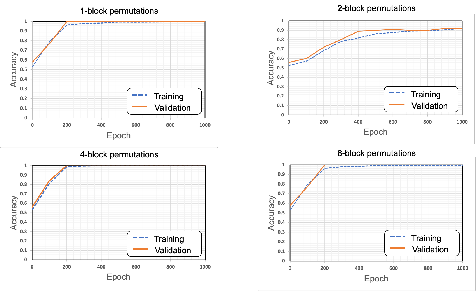
\includegraphics[width=1.0\columnwidth]{figures/SVGgraph_25stripe.pdf}
    \end{center}
    \vspace{-8pt}
	\caption{Accuracy curves of DNN for training and validation with datasets of two matrices with 0 and 1 values swapped every 25 columns.}
	\label{fig:accu_25stripe}
\end{figure}
%%%%%%%%%%%%%%%%%%%%%%%%%%%%

%%%%%%%%%%%%%%%%%%%%%%%%%%%%
\begin{figure}[t]
    \begin{center}
        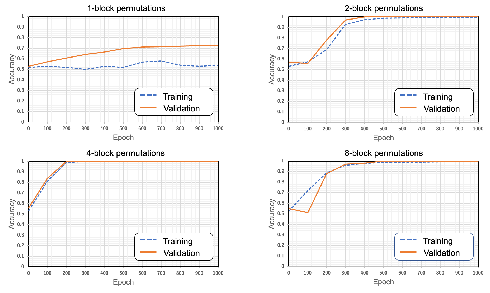
\includegraphics[width=1.00\columnwidth]{figures/SVGstripe_graph.pdf}
    \end{center}
    \vspace{-8pt}
	\caption{Accuracy curves of DNN for training and validation with datasets of two matrices with 0 and 1 values swapped per column.}
	\label{fig:accu_stripe}
\end{figure}
%%%%%%%%%%%%%%%%%%%%%%%%%%%%

%%%%%%%%%%%%%%%%%%%%%%%%%%%%
\begin{figure}[t]
    \begin{center}
        \includegraphics[width=0.8\columnwidth]{figures/graph_stripe_1block99ratio.pdf}
    \end{center}
    \vspace{-8pt}
	\caption{Accuracy curves of DNN for training and validation with datasets of two matrices with 0 and 1 values swapped in each column with a 1\% probability of shuffling two rows together and the rest shuffled row by row.}
	\label{fig:accu_stripe_1block99ratio}
\end{figure}
%%%%%%%%%%%%%%%%%%%%%%%%%%%%

%%%%%%%%%%%%%%%%%%%%%%%%%%%%
\begin{figure}[t]
    \begin{center}
        \includegraphics[width=0.8\columnwidth]{figures/graph_stripe_1block95ratio.pdf}
    \end{center}
    \vspace{-8pt}
	\caption{Accuracy curves of DNN for training and validation with datasets of two matrices with 0 and 1 values swapped per column with a 5\% probability of shuffling two rows together and the rest shuffled row by row.}
	\label{fig:accu_stripe_1block95ratio}
\end{figure}
%%%%%%%%%%%%%%%%%%%%%%%%%%%%

%%%%%%%%%%%%%%%%%%%%%%%%%%%%
\begin{figure}[t]
    \begin{center}
        \includegraphics[width=0.8\columnwidth]{figures/inkscape_graph_audio_8block.pdf}
    \end{center}
    \vspace{-8pt}
	\caption{Accuracy curves of DNN for training and validation with datasets of audio data shuffled into groups of 8 lines each.}
	\label{fig:accu_audio_8block}
\end{figure}
%%%%%%%%%%%%%%%%%%%%%%%%%%%%

%%%%%%%%%%%%%%%%%%%%%%%%%%%%
\begin{figure}[t]
    \begin{center}
        \includegraphics[width=0.8\columnwidth]{figures/inkscape_graph_audio_16block.pdf}
    \end{center}
    \vspace{-8pt}
	\caption{Accuracy curves of DNN for training and validation with datasets of audio data shuffled into groups of 16 lines each.}
	\label{fig:accu_audio_16block}
\end{figure}
%%%%%%%%%%%%%%%%%%%%%%%%%%%%


Fig.~\ref{fig:accu_01mat}〜Fig.~\ref{fig:accu_stripe}には,全ての成分が0と1の行列,25列毎に0と1の値が入れ替わる行列,1列毎に0と1の値が入れ替わる行列の周波数成分に対して
それぞれ1行,2行,4行,8行分をまとめてシャッフルを行った時の結果を示す.この結果から,各周波数成分の8行分をまとめてシャッフルした場合,実験を行った全てのパターンにおいてどれも正答率が100\%に近い値となっている.
しかし,1列毎に0と1の値が入れ替わる行列に対して各行ごとにシャッフルを行った場合は,正答率が54\%程度となった.即ち,提案手法において各行ごとにシャッフルを行なった行列に対してはパーミュテーション問題を解決することが難しいが,ブロック単位でのパーミュテーション問題は容易に解けると言える.
Fig.~\ref{fig:accu_stripe_1block99ratio}とFig.~\ref{fig:accu_stripe_1block95ratio}より,1列毎に0と1の値が入れ替わる行列に対して,95\%の割合で1行ごとにシャッフルしそれ以外は2行ごとにシャッフルした場合の正答率は93\%程度となったが,99\%の割合で1行ごとシャッフルしそれ以外は2行ごとにシャッフルした場合の正答率は60\%程度となった.
このことより,DNNは少しでもブロック単位でシャッフルが行われていると学習が容易となることがわかる.
Fig.~\ref{fig:accu_audio_8block}とFig.~\ref{fig:accu_audio_16block}より,音声データに対して8行ごとと16行ごとのブロック単位でのパーミュテーション問題として考え実験を行った結果,どちらのグラフでも正答率が80\%を超えた.



\clearpage




\clearpage
%----------------------------------------------
\section{本章のまとめ}
\label{sec:matome}
%----------------------------------------------
本章では,提案手法の有効性を確認するため,FDICAを適用した後のパーミュテーション行列を模倣した人工データと実際の音声データを用いて,実験を行った.
実験の結果より,人工データを用いたブロック単位でのパーミュテーション問題に対しては,どのような行列であっても100\%に近い確率で解決できることを示した.
実際の音声データに対しても,ブロック単位でシャッフルが行われていると80\%を超える正答率になることを示した.
次章では,本論文における総括とした結論を述べる.


%%%%% 第5章 %%%%%
\chapter{結言}
\label{chap:con}

本論文では,FDICAに伴うパーミュテーション問題の解決を目的とし,DNNを用いたパーミュテーション解決法を新たに提案した.
DNNの入力には,ミニ振幅スペクトログラム成分を用いた.テストデータに対してはDNNの入力となるミニ振幅スペクトログラムをストライド幅に従って,ずらしていくことで時間方向に対して多数決処理を行った.
また,誤差逆伝播の際に,スペクトログラム同士で平均二乗誤差を行いDNNのモデルを最適化した.
実験結果より,ブロック単位でのパーミュテーション問題に対しては提案手法を用いて正しく並び替えができることを示した.

最後に今後の展望を述べる.
本論文では,DNNを用いた3音源以上にも対応できる新しいパーミュテーション解決手法の可能性に注目しており,基礎的な実験を行ってきた.
ただ,実際に3音源以上での実験は行っていないことに加えて,実行時間や計算量等はあまり考慮されていない.
今回行った2音源での実験の拡張版として,今後は3音源以上に対する実験も行っていきたい.
また,リアルタイムでの音源分離に適用する場合は,DNNモデル及び損失取得時の計算アルゴリズムを改良する必要がある.


%%%%%%%%%%%%%%%%%%%%%%%%%%% 後付 %%%%%%%%%%%%%%%%%%%%%%%%%%%
\backmatter

%%%%% 謝辞 %%%%%
\chapter{謝辞}

本論文は,香川高等専門学校電気情報工学科北村研究室にて行われた研究に基づくものです.

まず,本研究を進めるにあたり,ご多忙のところ熱心に
ご指導くださいました指導教員の北村大地講師に心より感謝申し上げます.
北村大地講師には,論文執筆や研究に関する議論など,細部にわたるまで
丁寧にご指導いただきました.DNNの研究で用いるサーバーの増設等にも取り組んでいただき,日々の研究を効率良く行うことができました.心よりありがたくお礼申し上げます.

北村研究室の先輩である専攻科2年の岩瀬佑太氏,大藪宗一郎氏,梶谷奈未氏,渡辺瑠伊氏には,音源分離に関する基礎概念のご説明をはじめ,研究の進め方に関して数々のご支援をいただきました.
特に,北村研究室の先輩である専攻科2年の渡辺瑠伊氏には,
DNNに関するアドバイスやサーバー管理に関する知見をはじめ,数々のご支援とご助言をいただきました.心より感謝申し上げます.
また,北村研究室同期の川口翔也氏・細谷泰稚氏・村田佳斗氏,溝渕悠朔氏には,日頃のディスカッションのほか,
1年に亘る研究室生活を様々な面で支えていただきました.
ここに感謝申し上げます.

最後になりますが,現在に至るまで私の学生生活を金銭的に支え,
暖かく見守って下さった両親には感謝の念に堪えません.
これまで本当にありがとうございました.


%%%%% 参考文献(直接書く場合) %%%%%
\addcontentsline{toc}{chapter}{\bibname} % 参考文献を目次に表示
\begin{thebibliography}{99}
  \bibitem{Kitamura2016taslp}
  D.~Kitamura, N.~Ono, H.~Sawada, H.~Kameoka, and H.~Saruwatari,
  ``Determined blind source separation unifying independent vector analysis and nonnegative matrix factorization,''
  \emph{IEEE/ACM Transactions on Audio, Speech, and Language Processing}, vol. 24, no. 9, pp. 1626--1641, 2016.

  \bibitem{Kitamura2016IWAENC}
  D.~Kitamura, N.~Ono, H.~Saruwatari, Y.~Takahashi, and K. Kondo,
  ``Discriminative and reconstructive basis training for audio source separation with semi-supervised nonnegative matrix factorization,''
  \emph{in Proceedings of International Workshop on Acoustic Signal Enhancement}, 2016, pp. 1--5.
\end{thebibliography}

%%%%% 参考文献(BibTeXを使う場合) %%%%%
% \addcontentsline{toc}{chapter}{\bibname} % 参考文献を目次に表示
% \bibliography{ref_abb_full,references}

%%%%% 発表文献一覧 %%%%%
\input{publication/publication.tex}

%%%%%%%%%%%%%%%%%%%%%%%%%%% 付録 %%%%%%%%%%%%%%%%%%%%%%%%%%%
\appendix

%%%%% 付録A %%%%%
%---------------------------------
\chapter{Birkhoff--von~Neumannの定理}
\label{chap:vonNeumann}
%---------------------------------
サイズ$N$の正方行列$\bm{D}$が二重確率行列であるとき,$\bm{D}$はサイズ$N$の全てのパーミュテーション行列$\{\bm{P}_i\}_{i=1}^{N!}$の凸結合で表せる.
即ち,凸結合の係数$\sigma_i \geq 0$を用いて次式が成立する.
\begin{align}
    \bm{D} = \sum_{i=1}^{N!} \sigma_i \bm{P}_i
\end{align}
但し,$\sigma_i$は凸結合係数であるため,$\sum_{i=1}^{N!} \sigma_i = 1$を満たす.
%---------------------------------
\chapter{人工データに対する予測結果}
\label{chap:artificial}
%---------------------------------

\ref{chap:ex}章で掲載した人工データに対する実験結果の他にも,4行,8行毎に各周波数成分をシャッフルした場合の実験も行った.
以下に実験結果を掲載する.

%%%%%%%%%%%%%%%%%%%%%%%%%%%%
\begin{figure*}[!t]
    \centering
    \subfloat[Accuracy for training and validation data.]{\includegraphics[clip, width=4.5in]{figures/graph/01mat_4block.pdf}
    \vspace{-15pt}
    \label{fig:acc_01mat_4block}}
    \\
    \subfloat[Input matrices with permutation problem (upper) and permutation-aligned matrices using predicted results (bottom).]{\includegraphics[clip, width=5.0in]{figures/01mat_4block.pdf}
    \label{fig:spec_01mat_4block}}  
    \caption{Experimental results with $\gamma=4$ using artificial source matrices of Fig.~\ref{fig:01mat_spec}.}
    \label{fig:01mat_4block}
\end{figure*}
%%%%%%%%%%%%%%%%%%%%%%%%%%%%

%%%%%%%%%%%%%%%%%%%%%%%%%%%%
\begin{figure*}[!t]
    \centering
    \subfloat[Accuracy for training and validation data.]{\includegraphics[clip, width=4.5in]{figures/graph/25stripe_4block.pdf}
    \vspace{-15pt}
    \label{fig:acc_25mat_4block}}
    \\
    \subfloat[Input matrices with permutation problem (upper) and permutation-aligned matrices using predicted results (bottom).]{\includegraphics[clip, width=5.0in]{figures/25stripe_4block.pdf}
    \label{fig:spec_25mat_4block}}  
    \caption{Experimental results with $\gamma=4$ using artificial source matrices of Fig.~\ref{fig:25stripe_spec}.}
    \label{fig:25mat_4block}
\end{figure*}
%%%%%%%%%%%%%%%%%%%%%%%%%%%%

%%%%%%%%%%%%%%%%%%%%%%%%%%%%
\begin{figure*}[!t]
    \centering
    \subfloat[Accuracy for training and validation data.]{\includegraphics[clip, width=4.5in]{figures/graph/stripe_4block.pdf}
    \vspace{-15pt}
    \label{fig:acc_stripe_4block}}
    \\
    \subfloat[Input matrices with permutation problem (upper) and permutation-aligned matrices using predicted results (bottom).]{\includegraphics[clip, width=5.0in]{figures/stripe_4block.pdf}
    \label{fig:spec_stripe_4block}}  
    \caption{Experimental results with $\gamma=4$ using artificial source matrices of Fig.~\ref{fig:stripe_spec}.}
    \label{fig:stripe_4block}
\end{figure*}
%%%%%%%%%%%%%%%%%%%%%%%%%%%%

%%%%%%%%%%%%%%%%%%%%%%%%%%%%
\begin{figure*}[!t]
    \centering
    \subfloat[Accuracy for training and validation data.]{\includegraphics[clip, width=4.5in]{figures/graph/01mat_8block.pdf}
    \vspace{-15pt}
    \label{fig:acc_01mat_8block}}
    \\
    \subfloat[Input matrices with permutation problem (upper) and permutation-aligned matrices using predicted results (bottom).]{\includegraphics[clip, width=5.0in]{figures/01mat_8block.pdf}
    \label{fig:spec_01mat_8block}}  
    \caption{Experimental results with $\gamma=8$ using artificial source matrices of Fig.~\ref{fig:01mat_spec}.}
    \label{fig:01mat_8block}
\end{figure*}
%%%%%%%%%%%%%%%%%%%%%%%%%%%%

%%%%%%%%%%%%%%%%%%%%%%%%%%%%
\begin{figure*}[!t]
    \centering
    \subfloat[Accuracy for training and validation data.]{\includegraphics[clip, width=4.5in]{figures/graph/25stripe_8block.pdf}
    \vspace{-15pt}
    \label{fig:acc_25mat_8block}}
    \\
    \subfloat[Input matrices with permutation problem (upper) and permutation-aligned matrices using predicted results (bottom).]{\includegraphics[clip, width=5.0in]{figures/25stripe_8block.pdf}
    \label{fig:spec_25mat_8block}}  
    \caption{Experimental results with $\gamma=8$ using artificial source matrices of Fig.~\ref{fig:25stripe_spec}.}
    \label{fig:25mat_8block}
\end{figure*}
%%%%%%%%%%%%%%%%%%%%%%%%%%%%

%%%%%%%%%%%%%%%%%%%%%%%%%%%%
\begin{figure*}[!t]
    \centering
    \subfloat[Accuracy for training and validation data.]{\includegraphics[clip, width=4.5in]{figures/graph/stripe_8block.pdf}
    \vspace{-15pt}
    \label{fig:acc_stripe_8block}}
    \\
    \subfloat[Input matrices with permutation problem (upper) and permutation-aligned matrices using predicted results (bottom).]{\includegraphics[clip, width=5.0in]{figures/stripe_8block.pdf}
    \label{fig:spec_stripe_8block}}  
    \caption{Experimental results with $\gamma=8$ using artificial source matrices of Fig.~\ref{fig:stripe_spec}.}
    \label{fig:stripe_8block}
\end{figure*}
%%%%%%%%%%%%%%%%%%%%%%%%%%%%


\end{document}
